%%%%%%%%%%%%%%%%%%%%%%%%%%%%%%%%%%%%%%%%%%%%%%%%%%%%%%%%%%%%%%%%%%%%%%%%%%

% abnTeX2: Modelo de Trabalho Acadêmico em conformidade com 
% as normas da ABNT

%%%%%%%%%%%%%%%%%%%%%%%%%%%%%%%%%%%%%%%%%%%%%%%%%%%%%%%%%%%%%%%%%%%%%%%%%%

\documentclass[english, 
               brazil, 
               bsc] %Opções bsc (TCC) e msc (Mestrado)
               {dcomp-abntex2}


%%%%%%%%%%%%%%%%%%%%%%%%%%%%%%%%%%%%%%%%%%%%%%%%%%%%%%%%%%%%%%%%%%%%%%%%%%
% Área para adição de pacotes extras
%%%%%%%%%%%%%%%%%%%%%%%%%%%%%%%%%%%%%%%%%%%%%%%%%%%%%%%%%%%%%%%%%%%%%%%%%%

\usepackage{lipsum} %Retirar para a versão final do documento

%Utilize aqui seu pacote preferido para algoritmos
\usepackage[linesnumbered]{algorithm2e}
\usepackage{tabularx}

%%%%%%%%%%%%%%%%%%%%%%%%%%%%%%%%%%%%%%%%%%%%%%%%%%%%%%%%%%%%%%%%%%%%%%%%%%

%Compila o indice
\makeindex

\begin{document}

% Seleciona o idioma do documento (conforme pacotes do babel)
\selectlanguage{brazil}

% Retira espaço extra obsoleto entre as frases.
\frenchspacing 

%%%%%%%%%%%%%%%%%%%%%%%%%%%%%%%%%%%%%%%%%%%%%%%%%%%%%%%%%%%%%%%%%%%%%%%%%%
% ELEMENTOS PRÉ-TEXTUAIS
%%%%%%%%%%%%%%%%%%%%%%%%%%%%%%%%%%%%%%%%%%%%%%%%%%%%%%%%%%%%%%%%%%%%%%%%%%

\pretextual

\titulo{Proposta de Aplicação Mobile para Autocuidado de Diabéticos com Acuidade Visual Prejudicada} 
\autor{Jonathan Kelvin de Jesus Santos}
\orientador{Profa. Dra. Adicinéia Aparecida de Oliveira}
\curso{Sistemas de Informação}

\inserirInformacoesPDF

\imprimircapa
% \imprimirfolhaderosto*

% \begin{dedicatoria}
   \vspace*{\fill}
   \centering
   \noindent
   \textit{Este trabalho é dedicado a todos que acreditam na educação\\
   como meio essencial para o desenvolvimento sustentável de qualquer sociedade.} \vspace*{\fill}
\end{dedicatoria}
% ---
%\begin{agradecimentos}

Não haveria como não falar da minha mãe, Diana, em primeiro lugar neste espaço,
esta que abriu mão de diversas coisas para lutar pelo bem de seus 3 filhos, que sempre quis o melhor
pra mim e fez o que pôde para evitar e alertar sobre meus erros. E mesmo não entendendo minhas escolhas,
não as barrou e sempre esteve lá para quando eu quebrasse a cara.

Mãe, obrigado por tudo!

Agradeço também à Sergiane e Walesson, que me confiaram a honra de ser padrinho de Walace.
Aos meus irmãos Daiane e David que, em meio à tantas brigas, sempre nos apoiamos e defendemos uns aos outros.
Ao meu primo, Lucas, que foi uma referência durante a graduação. E, ao restante dessa grande família que, embora
não os nomeie aqui, quero que saibam que foram e são muito importantes para mim.

As amizades que fiz foi o que me manteve firme para seguir até o final dessa jornada. Assim, não posso deixar de mencionar
Abayomi com quem tenho quilômetros de mensagens trocadas no Telegram e que está em constante mudança e revolta (\emph{pelu idi}).
Brunna que talvez não saiba, mas nos momentos em que eu estava cheio de ansiedade, fez-me sentir em paz,
enquanto lia livros no silêncio de sua sala.

Igor e seus argumentos socráticos que foram interpretados como sofistas e Geovanne que está trabalhando feito louco e
me deixando preocupado com um \emph{burnout}. Mayara que sempre notava quando estava desanimado e estava lá para quando
eu precisasse desabafar. Raul de quem eu tinha que esconder a preocupação para evitar que infartasse e, por fim devido
à ordem alfabética, Roberto, o tiozão do pavê.

Embora eu consciência de minhas dificuldades para me expressar, principalmente com relação a sentimentos,
não sei o por que, mas nunca consegui dizer ``Eu te amo'' para ninguém depois que cresci, nem mesmo para minha mãe.
Assim, queria aproveitar esse momento para aqui deixar registrado que embora nunca tenha-os dito:

Amo vocês!

Não posso esquecer dos professores do DComp que apresentaram os caminhos que possibilitaram que eu seguisse nessa jornada.
Também aos professores de outros departamentos como o DPS e DCS que mostraram a importância do pensamento crítico.
E, em especial, a Gilton sempre animado e com novas ideias, Leonardo por seus conselhos e desafios, e Ricardo que nos ouvia
e parecia entender nossas frustrações.

E, por fim, à minha orientadora Adicinéia que, além da orientação e paciência comigo neste trabalho,
foi a única que, transmitindo conhecimento durante as aulas, conseguiu manter minha concentração por tanto tempo,
horas, sem me dar sono.

\end{agradecimentos}
% ---
%\begin{epigrafe}[]
    \vspace*{\fill}
	\begin{flushright}
	
		\textit{Num processo de construção, de capital\\
				Esquecemos de algo vital, a inclusão\\
				E promovemos a exclusão, digital\\
				}
		
	\end{flushright}
\end{epigrafe}
% ---
%% resumo em português
\setlength{\absparsep}{18pt} % ajusta o espaçamento dos parágrafos do resumo
\begin{resumo}
    O \emph{Diabetes Mellitus} (DM) é um grupo de doenças endocrinológicas crônicas caracterizado pela elevação
    da glicose no sangue que requer cuidados médicos contínuos para redução de risco e controle glicêmico, e vem se
    tornando um desafio cada vez maior devido ao rápido aumento do número de casos nos últimos 20 anos. Com isso,
    complicações do DM já são a maior causa de cegueira em adultos de países desenvolvidos, sendo que pelo menos 2,2
    bilhões de pessoas no mundo vivem com deficiência visual (DV) em algum grau.
    Estudos anteriores identificaram a importância do autocuidado no tratamento do DM, a dificuldade
    no acesso a informações a respeito por pacientes com DV e as principais funcionalidades utilizadas
    como solução no mercado. Além disso, neste trabalho foi constatado que, mesmo com o aumento da informatização e
    popularização dos \emph{smartphones}, pessoas com DV ainda enfrentam sérias dificuldades devido à falta
    de acessibilidade em aplicações móveis. Perante o exposto, foi realizado um processo de Mapeamento Sistemático da
    Literatura (MSL) para estabelecer as técnicas de acessibilidade que poderiam ser adotadas no desenvolvimento
    de um aplicativo móvel chamado DiaVision. Assim, o aplicativo foi desenvolvido para Android e iOS, atendendo
    aos requisitos identificados para este público-alvo e soluções de acessibilidade encontradas no MSL\@.
    Uma versão inicial do \emph{app} foi avaliada por 77 pacientes com DV e os resultados desse estudo
    mostraram que 90,1\% dos participantes gostariam de ter o \emph{app}, com 62,3\% avaliando-o com nota máxima.
    Contudo, parte das soluções de acessibilidade foram implementadas após a realização desse estudo, assim,
    35,1\% dos participantes apontaram que o aplicativo precisava de melhorias quanto à acessibilidade. Dessarte,
    trabalhos futuros devem realizar uma nova avaliação do aplicativo com as novas funcionalidades e melhorias
    relativas à acessibilidade.

    \textbf{Palavras-chave}: aplicativo móvel. diabetes mellitus. autocuidado. acessibilidade. deficiência visual.
\end{resumo}
%% resumo em inglês
\setlength{\absparsep}{18pt} % ajusta o espaçamento dos parágrafos do resumo
\begin{resumo}[Abstract]
  \begin{otherlanguage*}{english}
    Diabetes Mellitus (DM) is a group of chronic endocrine diseases characterized by elevated blood
    glucose that requires continuous medical care for risk reduction and glycemic control, and has become
    an increasing challenge due to the rapid increase in the number of cases in the last 20 years. As a result,
    complications from DM are already the leading cause of blindness in adults in developed countries, with at
    least 2.2 billion people in the world living with visual impairment (VI) to some level. Previous studies
    have identified the importance of self-care in the treatment of DM, the difficulty in accessing information
    about it by patients with VI and the main features used as a solution in the market. Furthermore, in this
    work it was found that even with the increase in computerization and popularization of smartphones,
    people with VI still face serious difficulties due to the lack of accessibility in mobile applications.
    Therefore, a Systematic Literature Mapping (SLM) process was carried out to establish accessibility
    techniques that could be adopted in the development of a mobile application called DiaVision. Thus,
    the application was developed for Android and iOS, meeting the requirements identified for this target
    audience and accessibility solutions found in SLM\@. An initial version of the app was
    evaluated by 77 patients with VI and the results of this study showed that 90.1\% of the participants
    would like to have the app, with 62.3\% evaluating it with full mark. However, part of the
    accessibility solutions were implemented after this study was carried out, so 35.1\% of the
    participants pointed out that the application needed improvements in terms of accessibility. With
    this, future works must carry out a new evaluation of the application with the new functionalities
    and improvements related to accessibility.

    \textbf{Keywords}: mobile app, diabetes mellitus, self-care, accessibility, visual impairment.
  \end{otherlanguage*}
\end{resumo}


% \mostrarlistadeILUSTRACOES
% \mostrarlistadeQUADROS
% \mostrarlistadeTABELAS
%\mostrarlistadeCODIGOS
%\mostrarlistadeALGORITMOS
 
% Lista de abreviaturas e siglas

\begin{siglas}
  	\item[API]{\textit{Application Programming Interface}}
  	\item[DCOMP]{Departamento de Computação}
  	\item[DM]{\textit{Diabetes Mellitus}}
  	\item[\emph{Dev}]{\textit{Developer}}
  	\item[DV]{Deficiência Visual}
  	\item[DVP]{Deficiência Visual Parcial}
  	\item[DVT]{Deficiência Visual Total}
  	\item[eMag]{Modelo de Acessibilidade em Governo Eletrônico}
  	\item[IBGE]{Instituto Brasileiro de Geografia e Estatística}
  	\item[OMS]{Organização Mundial da Saúde}
  	\item[PDV]{Pessoa(s) com Deficiência Visual}
  	\item[TA]{Tecnologias Assistivas}
  	\item[TTS]{\textit{Text-to-speech}}
  	\item[SO]{Sistema Operacional}
	\item[UFS]{Universidade Federal de Sergipe}
  	\item[UX]{\textit{User Experience}}
  	\item[WHO]{\textit{World Health Organization}}
  	\item[W3C]{\textit{World Wide Web Consortium}}
\end{siglas}
%\include{Pre_Textual/Simbolos}
    
\mostrarSUMARIO

%%%%%%%%%%%%%%%%%%%%%%%%%%%%%%%%%%%%%%%%%%%%%%%%%%%%%%%%%%%%%%%%%%%%%%%%%%
% ELEMENTOS TEXTUAIS
%%%%%%%%%%%%%%%%%%%%%%%%%%%%%%%%%%%%%%%%%%%%%%%%%%%%%%%%%%%%%%%%%%%%%%%%%%

\textual
\chapter{Introdução}

% ---
\section{Contextualização e Motivação}
% ---

O Diebetes Mellitus (DM) vem se tornando um desafio global de saúde pública cada vez maior por conta do rápido aumento no número de casos nos últimos
20 anos \cite{ADA2019}.
Estimativas da Federação Internacional de Diabetes (IDF), do Atlas da Diabetes\footnote{\url{https://diabetesatlas.org/}}
de 2019, apontaram que 463 milhões de pessoas no mundo viviam com DM, o que representa cerca de 9.3\% da população
global adulta, e é esperado um aumento para 10,2\% (578 milhões) em 2030 e 10,9\% (700 milhões) em 2045 \cite{SAEEDI2019107843}.

O Brasil é o 5º país com mais diabéticos no mundo com 16,8 milhões em 2019, na faixa etária de 20 à 79 anos, e estimativas
de 21,5 e 26 milhões de casos para 2030 e 2045, respectivamente \cite{SAEEDI2019107843}. Os custos totais de hipertensão, diabetes
e obesidade no Sistema Único de Saúde (SUS) alcançaram 3,45 bilhões de reais em 2018, sendo 30\% desse custo relacionado ao DM \cite{Nilson2020}.

Já a retinopatia diabética é uma complicação vascular do diabetes, cuja prevalência está diretamente relacionada à duração
do diabetes e ao controle do nível de glicemia \cite{Solomon412}. Essa complicação é a maior causa de novos casos de cegueira
em adultos, na faixa etária de 20 à 74 anos, em países desenvolvidos \cite{ADA2019}. Além disso, outros distúrbios oculares
como o glaucoma e a catarata ocorrem mais cedo e com maior frequência em diabéticos \cite{ADA2019}.

Assim, atualmente o mundo enfrenta um sério problema com relação a saúde da visão. Segundo a Organização Mundial da Saúde (OMS),
pelo menos 2,2 bilhões de pessoas no mundo vivem com deficiência visual (DV) em algum grau, com isso,
a necessidade de cuidados com os olhos tende a crescer drasticamente nas próximas décadas \cite{WHO2019}.

Segundo a Associação Americana de Diabetes (ADA), serviços de educação e apoio para o autogerenciamento do diabetes
(DSMES, do inglês \emph{diabetes self-management education and support}) facilitam na aquisição de conhecimento e habilidades
necessárias para o autocuidado, incorporando as necessidades, objetivos e experiências de diabéticos \cite{ADA2019}. Portanto, DSMES
visam auxiliar o empoderamento dos pacientes com diabetes na tomada de decisões informadas de autogerenciamento \cite{Marrero2013}.

De acordo com estimativas de 2019, mais de 5 bilhões de pessoas no mundo possuem dispositivos móveis, sendo mais da metade destes, \textit{smartphones}
\cite{Taylor2019}. Embora, segundo \citeonline{morris2017smartphone}, cerca de 84\% da população estadunidense com DV possua ou utilize telefone celular,
a taxa média de indivíduos que possuem nos países menos desenvolvidos é de apenas 61\% \cite{ITU_2021}.

No Brasil, a taxa de adultos que relataram possuir dispositivos móveis foi de 83\% no total e 60\% para \textit{smartphones},
sendo que, na faixa etária entre 18 e 34 anos, houve um aumento no número de proprietários de \textit{smartphones} de
61\% em 2015 para 85\% em 2018 \cite{Taylor2019}.

\citeonline{Yan2019} elaboram um estudo abrangente, realizado com 479 \textit{apps} de 23 categorias da
\emph{Google Play}, utilizando uma ferramenta automatizada, o IBM \textit{Mobile Accessibility Checker}
(MAC), para encontrar possíveis problemas com acessibilidade relacionadas à DV nesses \textit{apps},
categorizando-os em V (Violação), PV (Potencial Violação) e A (Alerta). Os resultados mostraram que 94.8\%, 97.5\% e 66.4\% dos apps continham problemas
relacionados à V, PV e A, respectivamente \cite{Yan2019}.

Diante da popularização dos \emph{smartphones} e das problemáticas mencionadas, o presente trabalho visa desenvolver uma aplicação móvel
com DSMES, para ao autocuidado de diabéticos, considerando a resolução dos principais problemas de acessibilidade para pessoas com
deficiência visual (PDV).

% ---
\section{Objetivos}
% ---

Nesta seção são apresentados os objetivos, divididos em geral e específicos. Onde o objetivo geral dá uma visão mais ampla sobre o objeto
de estudo e os específicos visam aprofundar as intenções expressas no geral \cite{cervo2006metodologia}.

% ---
\subsection{Geral}
% ---

O objetivo deste trabalho é desenvolver uma aplicação móvel multiplataforma e assistiva voltada ao autocuidado de pessoas com diabetes
e acuidade visual prejudicada. Implementando soluções para os principais problemas de acessibilidade à PDV na utilização de aplicativos móveis.

% ---
\subsection{Específicos}
% ---

Para atingir objetivo deste trabalho, os seguintes objetivos específicos foram definidos:

\begin{itemize}
    \item Identificar os principais problemas enfrentados por PDV na utilização de aplicações móveis;
    \item Identificar as principais técnicas e soluções de acessibilidade à PDV para aplicações móveis;
    \item Relacionar as principais técnicas e soluções identificadas aos principais problemas identificados;
    \item Realizar o desenvolvimento do aplicativo móvel com os principais requisitos levantados;
    \item Aplicar as soluções identificadas para os principais problemas de acessibilidade ao aplicativo.
\end{itemize}

% ---
\section{Metodologia}
% ---

A metodologia adotada neste estudo foi a quantitativa exploratória, visando responder as questões de pesquisa apresentadas
no início do capítulo 3, assim, obtendo maior familiaridade com o problema e possíveis soluções.

Para isso, foi realizado um levantamento bibliográfico por meio de um Mapeamento Sistemático da Literatura (MSL), onde foi possível
realizar uma análise dos resultados dos estudos selecionados (de acordo com o protocolo) e dos relacionados (estudos de mapeamento).

% ---
\section{Organização do Documento}
% ---
Neste capítulo foram apresentados a contextualização, a motivação e os objetivos deste trabalho. Bem como, a metodologia adotada.

Para facilitar a navegação e melhor entendimento, este documento está organizado em capítulos, cujas descrições são listadas a seguir:
\begin{itemize}
    \item Capítulo 2 - Fundamentação Teórica: aborda os principais conceitos relacionados ao trabalho realizado;
    \item Capítulo 3 - Mapeamento Sistemático da Literatura: descreve os estudos selecionados e os relacionados, e apresenta uma análise dos resultados;
    \item Capítulo 4 - Plano de continuidade: descreve o que será realizado e apresenta o cronograma das próximas etapas deste trabalho.
\end{itemize}

\chapter{Fundamentação Teórica}

Neste capítulo...

% ---
\section{Diabetes Mellitus}
% ---

De acordo com a Associação Americana de Diabetes (ADA), o Diabetes Mellitus (DM) é um grupo de doenças endocrinológicas crônicas
caracterizado pela elevação da glicose no sangue, devido à deficiência de ação do hormônio insulina, que requer cuidados médicos
contínuos para redução de risco e controle glicêmico \cite{ADA2019}.

O DM possui dois tipos, onde o tipo 1 afeta a produção de insulina devido à uma reação autoimune às proteínas das células das
ilhotas do pâncreas e o tipo 2 afeta o processamento do açúcar no sangue e é causado por fatores genéticos relacionados à
secreção prejudicada de insulina, resistência à insulina e fatores ambientais, como obesidade, alimentação excessiva, falta de
exercício, estresse e o envelhecimento \cite{Ozougwu_2013}.

A diabetes vem se tornando um desafio global de saúde pública cada vez maior por conta do rápido aumento no número de casos.
Estimativas da Federação Internacional de Diabetes (IDF), através do Atlas da Diabetes\footnote{\url{https://diabetesatlas.org/}}
de 2019, apontaram que 463 milhões de pessoas no mundo viviam com DM, o que representa cerca de 9.3\% da população
global adulta, e é esperado um aumento para 10,2\% (578 milhões) em 2030 e 10,9\% (700 milhões) em 2045 \cite{SAEEDI2019107843}.

O Brasil é o 5º país com mais diabéticos no mundo com 16,8 milhões em 2019, na faixa etária de 20 à 79 anos, e estimativas
de 21,5 e 26 milhões de casos para 2030 e 2045, respectivamente \cite{SAEEDI2019107843}. Os custos totais de hipertensão, diabetes
e obesidade no Sistema Único de Saúde (SUS) alcançaram 3,45 bilhões de reais em 2018, sendo 30\% desse custo relacionado ao DM \cite{Nilson2020}.

Já a retinopatia diabética é uma complicação vascular do diabetes, cuja prevalência está diretamente relacionada à duração
do diabetes e ao controle do nível de glicemia \cite{Solomon412}. Essa complicação é a maior causa de novos casos de cegueira
em adultos, na faixa etária de 20 à 74 anos, em países desenvolvidos \cite{ADA2019}. Além disso, outros distúrbios oculares
como o glaucoma e a catarata ocorrem mais cedo e com maior frequência em diabéticos \cite{ADA2019}.

Os resultados de uma metanálise realizada no estudo de \citeonline{AMINUDDIN2021103286} apontaram que as intervenções
de autogerenciamento baseadas em \emph{smartphones} pareceram ter efeitos benéficos sobre atividades de autocuidado para
pacientes com DM tipo 2.

% ---
\section{Deficiência visual}
% ---

De acordo com a Classificação Internacional de Funcionalidade, Incapacidade e Saúde (ICF),
a incapacidade enfrentada por pessoas com deficiência visual (PDV) não é determinada apenas
pela condição ocular, mas também pelo ambiente físico e social em que a pessoa vive, bem como
as dificuldades que pode enfrentar para realização de atividades como autocuidado, os problemas
que sofrem cotidianamente, como em ir para o trabalho ou escola, e o acesso a cuidados, produtos
e serviços oftalmológicos \cite{WHO2019}.

Assim, atualmente o mundo enfrenta um sério problema com relação a saúde da visão. Segundo a Organização Mundial da Saúde (OMS),
pelo menos 2,2 bilhões de pessoas no mundo vivem com deficiência visual (DV) em algum grau, com isso
a necessidade de cuidados com os olhos tende a crescer drasticamente nas próximas décadas \cite{WHO2019}.

O estudo da \citeonline{WHO2019} aponta que mais de 1 bilhão dos casos de pessoas com DV poderiam ser prevenidos ou
tratados. Ainda segundo esse estudo, os principais motivos para esses casos são:

\begin{itemize}
    \item O tempo despendido em ambientes fechados e aumento das atividades \textit{"near work"} (ler, escrever, assistir TV, jogar videogames, etc);
    \item O aumento no número de pessoas vivendo com diabetes, principalmente o tipo 2;
    \item Muitas pessoas não terem acesso a serviços oftalmológicos e verificações de rotina.
\end{itemize}

No Brasil, de acordo com o último censo do Instituto Brasileiro de Geografia e Estatistica (IBGE), realizado em 2010,
cerca de 18,6\% da população era afetada por algum tipo de DV, sendo 3,46\% por DV severa
\cite{IBGE2012}. Embora o próximo censo esteja previsto para 2022\footnote{\url{https://censo2022.ibge.gov.br/}}, outra pesquisa
foi realizada pelo Ministério da Saúde em 2019, a Pesquisa Nacional de Saúde (PNS), e apontou que 3,4\% da população brasileira,
com 2 ou mais anos de idade, possui muita dificuldade ou não enxerga \cite{stopa2020pesquisa}.

% ---
\section{Acessibilidade e Leitores de tela}
% ---

Segundo o Art. 3º da Lei Brasileira de Inclusão da Pessoa com Deficiência, acessibilidade se refere à:

\begin{citacao}
    possibilidade e condição de alcance para utilização, com segurança e autonomia, de espaços, mobiliários, equipamentos urbanos,
    edificações, transportes, informação e comunicação, \textbf{inclusive seus sistemas e tecnologias}, bem como de outros serviços e
    instalações abertos ao público, de uso público ou privados de uso coletivo, tanto na zona urbana como na rural, por pessoa com
    deficiência ou com mobilidade reduzida.
\end{citacao}

Acesso a Tecnologias Assistivas (AT) adequadas e de qualidade por um preço acessível melhora o funcionamento individual e
a independência, ao mesmo tempo que facilita a participação e integração na sociedade \cite{world2019global}.

Visando a inclusão das pessoas com DV, tecnologias conhecidas como Tecnologias Assistivas (TA) se tornam cada vez mais presentes.
\citeonline{Cook2014} utilizam em seu livro, uma definição de TA mundialmente utilizada que foi definida por uma \textit{Public Law}
dos Estados Unidos da América (EUA). Os autores justificam a utilização dessa definição por a mesma contemplar os pontos mais
importantes a respeito de TA, como diz a seguir:

\begin{citacao}
    Qualquer item, parte de equipamento ou sistema adquirido comercialmente, modificado ou customizado que é utilizado para aumentar, manter ou melhorar as capacidades
    funcionais de pessoas com deficiência \cite{Cook2014}.
\end{citacao}

Para que essas TAs funcionassem adequadamente, organizações como a \textit{World Wide Web Consortium} (W3C) definiram diretrizes que deveriam ser seguidas no desenvolvimento
de aplicações \textit{web} \cite{W3C2019}. Já para aplicações \textit{mobile}, como a implementação da tecnologia varia de acordo com o Sistema Operacional (SO), essa
definição se deu pelas próprias proprietárias dos SOs, tais como Google e Apple.

% ---
\section{Diretrizes de acessibilidade}
% ---

Um estudo realizado por \citeonline{Ballantyne2018}, compila um conjunto de diretrizes para acessibilidade \textit{mobile} e realiza
testes em 25 dos \textit{apps} mais populares da \emph{Google Play}. Os resultados do estudo revelaram que apenas 8 dos 25 selecionados
possuiam taxa de conformidade com as diretrizes acima de 75\%. O estudo ainda revela que 63\% das violações encontradas são
relacionadas ao \textit{design} (componentes de tela).

Já \citeonline{Yan2019} elaboram um estudo mais abrangente, realizado com 479
\textit{apps} de 23 categorias da \emph{Google Play}. Os autores utilizaram uma ferramenta automatizada, o IBM
\textit{Mobile Accessibility Checker} (MAC), para encontrar possíveis problemas com acessibilidade nesses \textit{apps},
categorizando-os em V (Violação), PV (Potêncial Violação) e A (Alerta). Os resultados mostraram
que 94.8\%, 97.5\% e 66.4\% dos apps continham problemas realacionados a V, PV e A, respectivamente \cite{Yan2019}.

Para \citeonline{Quispe2020} os principais fatores para a baixa priorização da acessibilidade de aplicações \textit{mobile}
são o desconhecimento, a alta demanda e a falta de tempo das equipes de desenvolvimento, fazendo com que se concentrem nos
requisitos funcionais em detrimento de requisitos não funcionais de usabilidade como o de acessibilidade.

% ---
\section{Desenvolvimento de aplicações multiplataforma}
% ---

Segundo  as estimativas, mais de 5 bilhões de pessoas possuem dispositivos móveis no mundo, sendo mais da metade destes, \textit{smartphones}.
No Brasil, a taxa de adultos que dizem possuir dispositivos móveis é de 83\% no total e 60\% para \textit{smartphones}. Na faixa etária entre 18
e 34 anos, houve um aumento no número de proprietários de \textit{smartphones} de 61\% em 2015 para 85\% em 2018 \cite{Taylor2019}. //CETIC.br, NIC-BR, ITU (ONU)

\chapter{Mapeamento Sistemático}
Este capítulo abordará o processo de Mapeamento Sistemático adotado neste estudo, com o objetivo de levantar métodos, técnicas e padrões utilizados na implementação de acessibilidade em aplicações \emph{mobile}.


\section{Protocolo de Mapeamento Sistemático}
O termo Mapeamento Sistemático da Literatura (MSL) se refere a uma revisão ampla de estudos primários existentes em um tema específico e visa identificar as evidências disponíveis nessa área \cite{Kitchenham2007}.
O método de Mapeamento Sistemático adotado foi o de Kitchenham, descrito em \citeonline{Silva2009}.
De acordo com o método, foi desenvolvido um protocolo de revisão com intuito de responder as seguintes questões:
\begin{enumerate}
\item Quais são as principais técnicas, padrões e métodos utilizados no desenvolvimento de aplicações móveis acessíveis para deficientes visuais?
\item Quais são as tecnologias utilizadas no desenvolvimento dessas soluções?
\item Para quais plataformas as soluções foram propostas?
\item Quais são os públicos alvos dessas soluções?
\end{enumerate}

O \emph{Parfisal}\footnote{\url{https://parsif.al/}}, ferramenta \emph{online} que auxilia no desenvolvimento de Revisões Sistemáticas da Literatura, foi utilizado neste estudo.
Com ele foi possível importar os resultados das buscas nas bases, identificar os artigos duplicados, definir os critérios para inclusão e exclusão, realizar a seleção dos estudos e, por fim, obter os relatórios para construção dos artefatos que apresentam o processo e os resultados desse MSL.

\subsection{Bases de Dados}
Cinco bases de dados científicos foram escolhidas neste trabalho, a \emph{IEEE Xplore}\footnote{\url{https://ieeexplore.ieee.org}}, onde estão disponíveis conteúdos técnicos e científicos publicados pelo \emph{Institute of Electrical and Electronics Engineers (IEEE)} e seus parceiros,
a \emph{Scopus}\footnote{\url{https://www.scopus.com}}, que é mantida pela \emph{Elsevier} e combina um abrangente banco de dados de resumos e citações de literatura acadêmica em diversas áreas, a \emph{ScienceDirect}\footnote{\url{https://www.sciencedirect.com}}, principal plataforma da \emph{Elsevier} de literatura revisada por pares,
a \emph{ACM Digital Library}\footnote{\url{https://dl.acm.org}}, uma plataforma de pesquisa que conta com textos completos de todas as publicações da \emph{Association for Computing Machinery (ACM)} e de uma curada coleção de publicações de editoras selecionadas e a \emph{PubMed}\footnote{\url{https://pubmed.ncbi.nlm.nih.gov}},
plataforma gratuita que conta com uma base de dados com mais de 33 milhões de citações e resumos da literatura biomédica.

\subsection{\emph{String} de Busca}
Para realização da busca dos artigos, um conjunto de palavras-chave e sinônimos foi definido de acordo com o tema deste trabalho, como é mostrado no \autoref{qua-pal-sin}.

\begin{quadro}[htb]
\caption{\label{qua-pal-sin}Palavras-chave e Sinônimos.}
\begin{tabular}{|c|c|}
  %\hline
    \hline
   \textbf{Palavra-chave} & \textbf{Sinônimos (Inglês)} \\ \hline
    Acessibilidade & \emph{Accessibility} \\ \hline
    Aplicativo & \emph{Application, App} \\ \hline
    Deficiência visual & \emph{Visual impairment, Visually impaired} \\ \hline
    Móvel & \emph{Mobile, Smartphone} \\ \hline
   % \hline
\end{tabular}
\legend{Fonte: Autor}
\end{quadro}

Com o objetivo de manter a consistência da busca nas diferentes bases, foi gerada, a partir das palavras-chave, a \emph{string} de busca genérica indicada no \autoref{qua-str-gen}.
As palavras-chave que possuem sinônimos aparecem na \emph{string} entre parêntesis com o operador \emph{OR}, visando incluir os resultados que contenham um dos termos, para indicar que esses termos são sinônimos no contexto do tema abordado neste trabalho.

\begin{quadro}[htb]
\caption{\label{qua-str-gen}\emph{String} genérica.}
\begin{tabular}{|m{11.5cm}|}
  %\hline
    \hline
    \textbf{\emph{String} genérica} \\
    \hline
    \emph{accessibility AND (“visual impairment” OR “visually impaired”) AND (mobile OR smartphone) AND (app OR application)} \\ \hline
   % \hline
\end{tabular}
\legend{Fonte: Autor}
\end{quadro}

A \emph{string} genérica serviu de modelo para criação das \emph{strings} específicas, indicadas no \autoref{qua-str-esp}, de acordo com as particularidades de cada base de busca.
As \emph{strings} específicas buscam pelas palavras-chave nos títulos e resumos dos artigos, afim de encontrar os que focam no tema proposto neste estudo, não considerando os que apenas citam as palavras-chave ao longo texto.

\begin{quadro}[htb]
\caption{\label{qua-str-esp}\emph{Strings} específicas para busca em cada base.}
\begin{tabular}{|m{3.5cm} | m{11.5cm}|}
   \hline
   \textbf{Base} & \textbf{\emph{String} de busca} \\ \hline
    \emph{ACM Digital Library} & \emph{(Abstract:(accessibility) OR Title:(accessibility)) AND (Abstract:("visual impairment" OR "visually impaired") OR Title:("visual impairment" OR "visually impaired")) AND (Abstract:(smartphone OR mobile) OR Title:(smartphone OR mobile)) AND (Abstract:(app OR application) OR Title:(app OR application))} \\ \hline
    \emph{IEEE Xplore} & \emph{(("Abstract":accessibility OR "Document Title":accessibility) AND ("Document Title":mobile OR "Document Title":smartphone OR "Abstract":mobile OR "Abstract":smartphone) AND ("Document Title":"visual impairment" OR "Abstract":"visual impairment" OR "Document Title":"visually impaired" OR "Abstract":"visually impaired") AND ("Document Title":app OR "Document Title":application OR "Abstract":app OR "Abstract":application))} \\ \hline
    \emph{PubMed} & \emph{(accessibility[Abstract] OR accessibility[Title]) AND ("visually impaired"[Abstract] OR "visual impairment"[Abstract] OR "visually impaired"[Title] OR "visual impairment"[Title]) AND (mobile[Abstract] OR smartphone[Abstract] OR mobile[Title] OR smartphone[Title]) AND (app[Title] OR app[Abstract] OR application[Title] OR application[Abstract])} \\ \hline
    \emph{ScienceDirect} & \emph{Title, abstract, keywords: accessibility AND ("visual impairment" OR "visually impaired") AND (mobile OR smartphone) AND (app OR application)} \\ \hline
    \emph{Scopus} & \emph{TITLE-ABS (accessibility AND ("visual impairment" OR "visually impaired") AND (smartphone OR mobile) AND (app OR application))} \\ \hline
\end{tabular}
\legend{Fonte: Autor}
\end{quadro}

A busca nas bases de dados selecionadas foi realizada no dia 04 de outubro de 2021 e retornou um total de 258 resultados.
Como mostra a \autoref{fig_art_enc}, a maior quantidade de resultados foi encontrada na \emph{Scopus}, isso acontece porque ela possui, de acordo com seu site\footnote{\url{https://www.elsevier.com/pt-br/solutions/scopus}}, o maior banco de dados de resumos e citações da literatura com revisão por pares.
Em seguida aparecem a \emph{ACM Digital Library} e a \emph{IEEE Xplore} cujas principais publicações são na área de computação, e elétrica no caso da IEEE\@.
Por fim, com as menores quantidades, a \emph{ScienceDirect}, com publicações nas mais diversas áreas da ciência e a \emph{PubMed} com publicações na área biomédica, justificando os menores resultados, visto que a busca foi realizada visando encontrar técnicas, métodos e padrões para o desenvolvimento de aplicações móveis acessíveis.

\begin{figure}[htb]
	\caption{\label{fig_art_enc}Quantidade de artigos encontrados por base.}
	\begin{center}
	    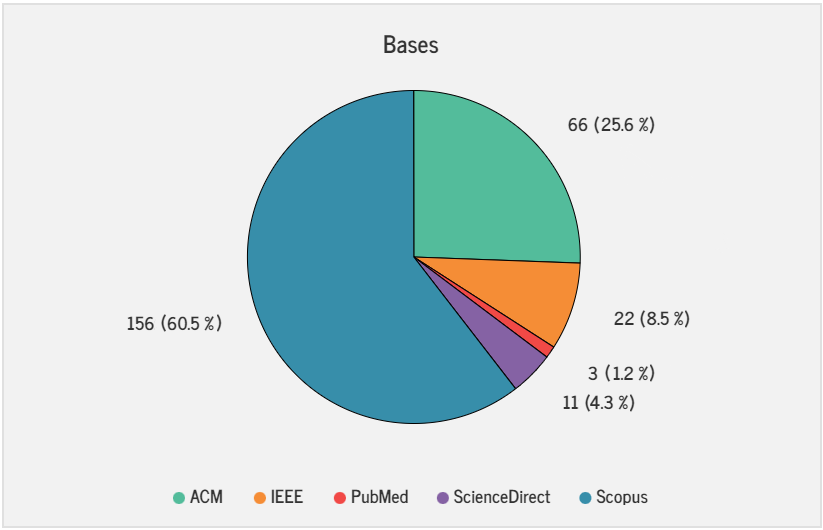
\includegraphics[scale=0.7]{Imagens/msl/artigos_encontrados.png}
	\end{center}
	\legend{Fonte: Autor}
\end{figure}

\subsection{Critérios de Inclusão e Exclusão}

Critérios de inclusão e exclusão foram definidos visando a coerência dos artigos selecionados com o tema deste trabalho, bem como a remoção de artigos incompletos ou indisponíveis.
Os critérios são:

\textbf{Critérios de Inclusão}
\begin{itemize}
  \item O artigo deve propor método, técnica ou padrão para o desenvolvimento de aplicações móveis com acessibilidade para deficientes visuais;
  \item O artigo deve estar disponível na \emph{web};
  \item O artigo deve apresentar texto completo em formato eletrônico;
  \item O artigo deve estar escrito em português ou inglês.
\end{itemize}

\textbf{Critérios de Exclusão}
\begin{itemize}
  \item O artigo não apresenta proposta de aplicação móvel como solução;
  \item O artigo não apresenta aplicativo desenvolvido no contexto do tema deste trabalho;
  \item O artigo é um livro ou parte de um;
  \item O artigo foi publicado antes de 2016;
  \item O artigo está incompleto, indisponível ou duplicado.
\end{itemize}

No processo de seleção dos estudos, inicialmente, foi aplicado o critério de exclusão de artigos duplicados e, em seguida, o de artigos publicados antes de 2016, rejeitando 48 e 65 artigos, respectivamente.
Esses critérios foram priorizados por não haver a necessidade da leitura dos títulos e resumos dos artigos para serem aplicados.
Por fim, após a leitura dos títulos e resumos, mais 112 artigos foram rejeitados, totalizando 225 artigos.
Assim, sendo aceitos 33 artigos para leitura completa e análise.
A \autoref{fig_res_sel} apresenta o resultado dessa seleção.

\begin{figure}[htb]
	\caption{\label{fig_res_sel}Quantidade de artigos aceitos, rejeitados e duplicados na seleção.}
	\begin{center}
	    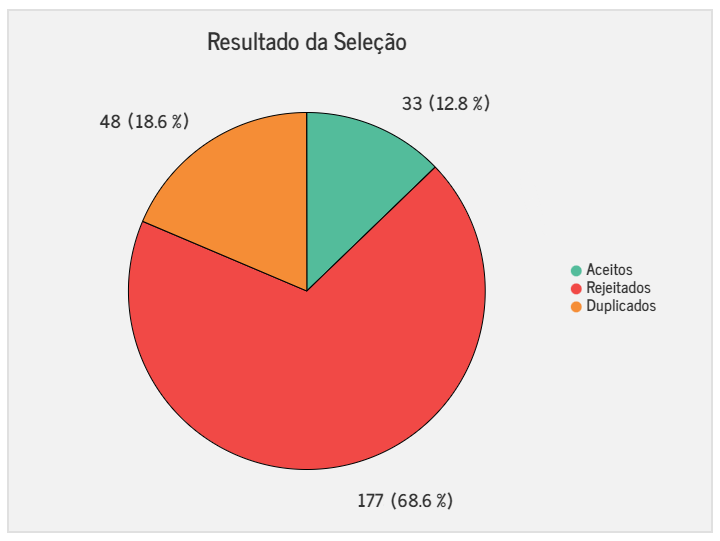
\includegraphics[scale=0.7]{Imagens/msl/resultado_selecao.png}
	\end{center}
	\legend{Fonte: Autor}
\end{figure}

A \autoref{fig_res_sel_base} mostra o resultado da seleção para cada base de busca.
Não houve priorização de bases ao rejeitar artigos duplicados, visto que a ferramenta utilizada possui uma funcionalidade que indica esses artigos, sendo necessário apenas a confirmação.
Com isso, algumas bases como a \emph{PubMed}, cujo resultado da busca retornou apenas 3 artigos sendo 1 duplicado, acabou apresentando poucos ou nenhum artigo aceito.

\begin{figure}[htb]
	\caption{\label{fig_res_sel_base}Quantidade de artigos aceitos e rejeitados por base.}
	\begin{center}
	    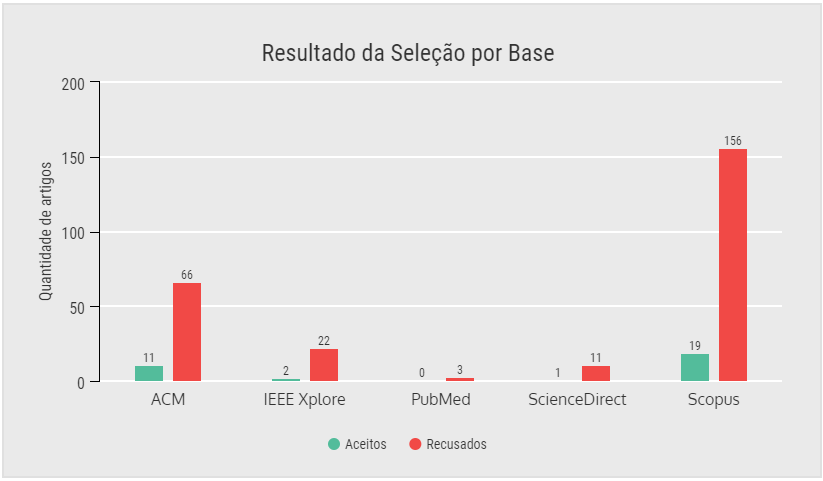
\includegraphics[scale=0.6]{Imagens/msl/resultado_selecao_base.png}
	\end{center}
	\legend{Fonte: Autor}
\end{figure}

\newpage

A frequência dos artigos rejeitados, de acordo com os critérios de exclusão, sendo que, para rejeição, o artigo deveria atender a pelo menos um desses critérios, pode ser observada no gráfico da \autoref{fig_art_rej}, onde é listada para cada critério.

\begin{figure}[htb]
	\caption{\label{fig_art_rej}Quantidade de artigos rejeitados por critério de exclusão.}
	\begin{center}
	    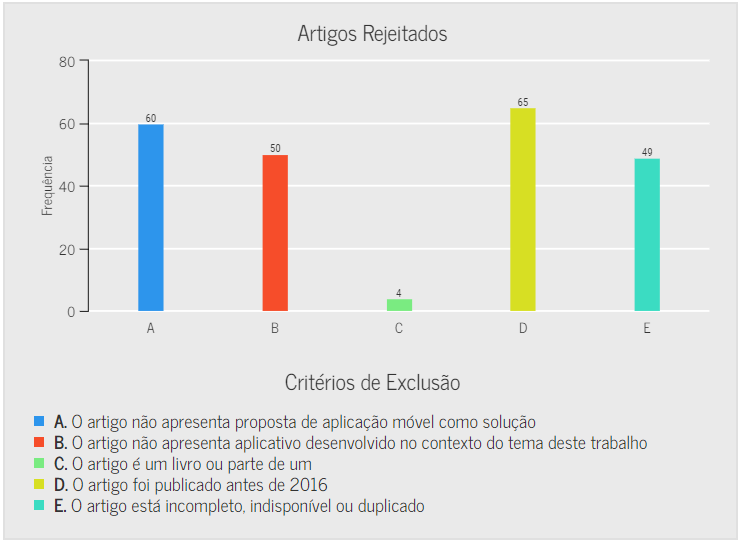
\includegraphics[scale=0.6]{Imagens/msl/artigos_rejeitados.png}
	\end{center}
	\legend{Fonte: Autor}
\end{figure}

Os critérios de exclusão levaram em consideração, principalmente, aspectos como divergência com o tema deste trabalho e não apresentação de aplicação desenvolvida para dispositivos móveis.
Os critérios D e E aparecem com grande frequência na \autoref{fig_art_rej}, valendo ressaltar a ordem na avaliação dos critérios (E, D, A, B e C), onde os artigos que se enquadraram em um dos critérios foram rejeitados, não sendo considerados para avaliação nos demais.
É comum que o critério D seja utilizado no próprio processo de busca dos artigos, filtrando apenas os anos de interesse, porém, como não foi possível adicionar esse filtro às \emph{strings} de busca para todas as bases, foi optado por não utiliza-lo, para manter a consistência nos resultados das buscas.

Após a aplicação dos critérios de exclusão, através da leitura e análise dos títulos e resumos, os artigos restantes, a priori, mostraram se enquadrar em todos os critérios de inclusão.
Assim, a \autoref{fig_art_act_ano} exibe a distribuição desses artigos por ano de publicação e base de busca, mostrando uma clara tendência de alta anual, nos últimos 5 anos, na quantidade de artigos que abordam o tema deste trabalho.
A base \emph{PubMed} foi desconsiderada nessa figura, visto que nenhum artigo dela foi selecionado como mostrou a \autoref{fig_art_rej}.


\begin{figure}[htb]
	\caption{\label{fig_art_act_ano}Quantidade de artigos aceitos por ano e base.}
	\begin{center}
	    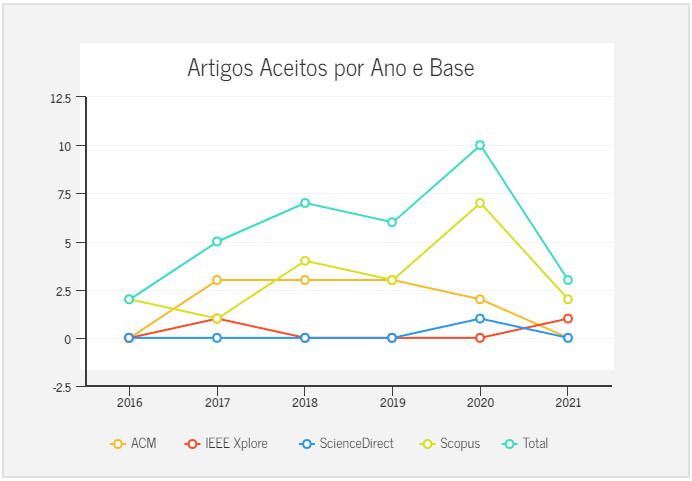
\includegraphics[scale=0.85]{Imagens/msl/artigos_aceitos_ano_base.png}
	\end{center}
	\legend{Fonte: Autor}
\end{figure}

\newpage{}

\subsection{Fase de Extração}

Durante a fase de extração, uma análise mais aprofundada dos artigos foi realizada, inicialmente com intuito de reaplicar os critérios já definidos e utilizados na fase anterior.
O resultado dessa última filtragem pode ser visto na \autoref{fig_fas_ext}.

\begin{figure}[htb]
	\caption{\label{fig_fas_ext}Artigos aceitos e rejeitados na fase de extração.}
	\begin{center}
	    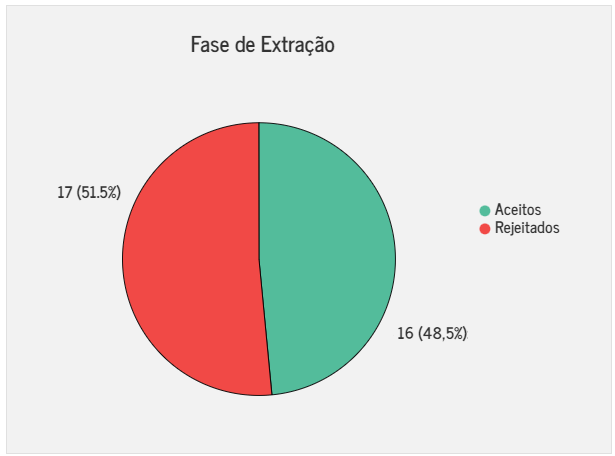
\includegraphics[scale=0.85]{Imagens/msl/fase_extracao_artigos.png}
	\end{center}
	\legend{Fonte: Autor}
\end{figure}

Como a aplicação inicial dos critérios foi realizada com base apenas na leitura dos títulos e resumos dos estudos, não foi possível garantir que os artigos aceitos realmente não se enquadravam nos critérios de exclusão.
Assim, com a análise mais aprofundada e leitura completa dos textos, foi possível identificar 18 artigos que se enquadravam em algum desses critérios, como mostrou a \autoref{fig_fas_ext}.

A \autoref{fig_art_rej_fas_ext} mostra a frequência de artigos que foram rejeitados por cada critério de exclusão.
Apenas os critérios com frequência maior que 0 foram considerados na figura.
O principal motivo para rejeição foi o B, onde os trabalhos apresentavam aplicações móveis que não haviam sido desenvolvidas com foco na acessibilidade da aplicação em si.
O segundo foi o A, onde os estudos não apresentavam uma aplicação móvel com acessibilidade à PDV como solução.

\begin{figure}[htb]
	\caption{\label{fig_art_rej_fas_ext}Artigos rejeitados na fase de extração por critério exclusão.}
	\begin{center}
	    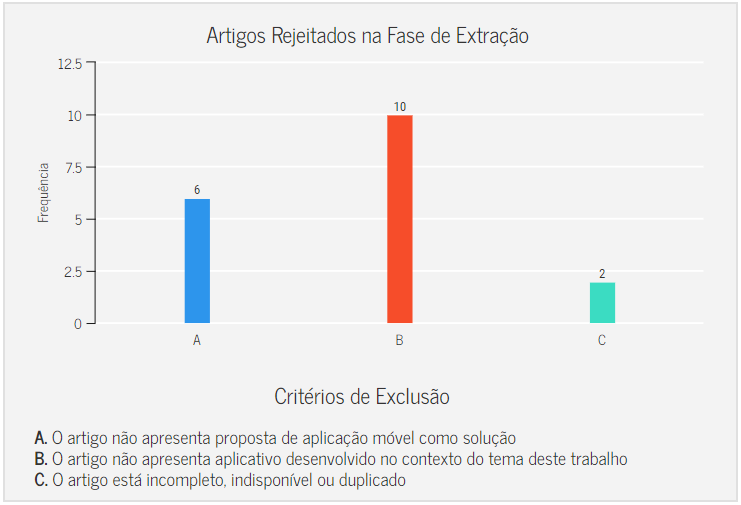
\includegraphics[scale=0.7]{Imagens/msl/artigos_rejeitados_fase_extracao.png}
	\end{center}
	\legend{Fonte: Autor}
\end{figure}

\newpage

Os 15 estudos aceitos na fase de extração, foram reunidos no \autoref{qua-art-ext} com a listagem de informações como o título do estudo, referência e o nome da base de dados em que o artigo foi encontrado.

\begin{quadro}[htb!]
\caption{\label{qua-art-ext}Artigos aceitos na fase de extração.}
\begin{tabular}{|m{0.8cm} | m{8.2cm} | m{2.7cm} | m{2.5cm}|}
  %\hline
    \hline
    \textbf{Sigla} &\textbf{Título} & \textbf{Referência} & \textbf{Base de dados} \\ \hline
    A1 & \emph{A Mobile Educational Game Accessible to All, Including Screen Reading Users on a Touch-Screen Device} & \cite{Leporini2017} & \emph{ACM Digital Library} \\ \hline
    A2 & \emph{A model-driven approach to cross-platform development of accessible business apps} & \cite{Christoph2020} & \emph{ACM Digital Library} \\ \hline
    A3 & \emph{An Accessible Roller Coaster Simulator for Touchscreen Devices: An Educational Game for the Visually Impaired} & \cite{Biase2018} & \emph{IEEE Xplore} \\ \hline
    A4 & \emph{Application for the Configuration and Adaptation of the Android Operating System for the Visually Impaired} & \cite{Oliveira2018} & \emph{ACM Digital Library} \\ \hline
    A5 & \emph{Blind and visually impaired user interface to solve accessibility problems} & \cite{Shera2021285} & \emph{Scopus} \\ \hline
    A6 & \emph{Design and development of a mobile app of drug information for people with visual impairment} & \cite{Amariles2020} & \emph{ScienceDirect} \\ \hline
    A7 & \emph{Designing multimodal mobile interaction for a text messaging application for visually impaired users} & \cite{Duarte2017} & \emph{Scopus} \\ \hline
    A8 & \emph{Do You like My Outfit? Cromnia, a Mobile Assistant for Blind Users} & \cite{Giuliana2018} & \emph{ACM Digital Library} \\ \hline
    A9 & \emph{Improved and Accessible E-Book Reader Application for Visually Impaired People} & \cite{Heesook2017} & \emph{ACM Digital Library} \\ \hline
    A10 & \emph{MathMelodies 2: A Mobile Assistive Application for People with Visual Impairments Developed with React Native} & \cite{Ducci2018} & \emph{ACM Digital Library} \\ \hline
    A11 & \emph{Object Recognition and Hearing Assistive Technology Mobile Application Using Convolutional Neural Network} & \cite{Caballero2020} & \emph{ACM Digital Library} \\ \hline
    A12 & \emph{QUIMIVOX MOBILE 2.0: Application for Helping Visually Impaired People in Learning Periodic Table and Electron Configuration} & \cite{Oliveira2019} & \emph{ACM Digital Library} \\ \hline
    A13 & \emph{``Talkin' about the weather'': Incorporating TalkBack functionality and sonifications for accessible app design} & \cite{Tomlinson2016377} & \emph{Scopus} \\ \hline
    A14 & \emph{Users’ perception on usability aspects of a braille learning mobile application ‘mBRAILLE’} & \cite{Nahar2019100} & \emph{Scopus} \\ \hline
    A15 & \emph{WordMelodies: Supporting Children with Visual Impairment in Learning Literacy} & \cite{Mascetti2019} & \emph{ACM Digital Library} \\ \hline
   % \hline
\end{tabular}
\legend{Fonte: Autor}
\end{quadro}
\newpage{}

\section{Resultados Encontrados}

Nesta seção, são apresentados os resumos com as principais características, relacionadas ao tema deste trabalho, dos artigos selecionados na fase de extração, visando encontrar respostas para as questões levantadas na definição do protocolo de MSL\@.

\subsection{\emph{A Mobile Educational Game Accessible to All, Including Screen Reading Users on a Touch-Screen Device}}

O estudo realizado por \citeonline{Leporini2017} teve o objetivo levantar informações e possíveis soluções para as dificuldades levantadas por um grupo composto por 6 pessoas cegas ao responder questões de tarefas interativas.
E investigou, através de tarefas interativas como exercícios e questionários, a acessibilidade e usabilidade de gestos e leitores de tela em dispositivos móveis com \emph{touch-screen}.

No artigo é apresentado um \emph{game mobile} que envolveu duas pessoas cegas com experiência na utilização de \emph{smartphones} na fase inicial do planejamento do protótipo.
O \emph{game} funciona como se fosse um ``sistema solar'' com oito planetas, onde cada planeta representa um conjunto de questões e exercícios.
O jogador recebe determinada pontuação cada vez que joga de acordo com os acertos e erros durante o game.
As principais funcionalidades do \emph{app} relativas à acessibilidade identificadas foram:

\begin{enumerate}
\item Contraste de cor para garantir diferentes níveis de acessibilidade;
\item Apresentações de conteúdos de forma auditiva e visual;
\item Interação via gestos ou toques;
\item Suporte auditivo com descrições dos elementos.
\end{enumerate}

Através da avaliação desse protótipo, por cegos, o estudo investigou o suporte de acessibilidade \emph{mobile} multiplataforma do conjunto de especificações técnicas, \emph{WAI-Aria}\footnote{\url{https://www.w3.org/WAI/standards-guidelines/aria/}}, observando problemas na detecção de elementos, devido às suas posições na tela e conteúdos difíceis de identificar na interação com leitores de tela.
Notando também que houve alguma dificuldade por conta de gestos implementados no \emph{app} diferirem dos habituais utilizados pelos usuários no \emph{VoiceOver} do \emph{iOS}.

Apesar dos problemas encontrados, o artigo aponta que o \emph{feedback} foi positivo e os resultados mostraram que os exercícios puderam ser realizados facilmente, por pessoas cegas, através de simples gestos com auxilio dos leitores de tela.

\textbf{Tecnologia utilizada para desenvolvimento:} \emph{Cordova Framework}.

\textbf{Plataforma alvo do \emph{app} desenvolvido:} multiplataforma (\emph{Android} e \emph{iOS}).

\textbf{Público alvo da aplicação:} PDV\@.

\subsection{\emph{A Model-Driven Approach to Cross-Platform Development of Accessible Business Apps}}

Um procedimento comum no processo de desenvolvimento de \emph{software} é considerar a acessibilidade para PDV apenas na etapa final.
Além disso, muitos desenvolvedores não estão cientes de técnicas de software para atender esse grupo, pois o domínio de apps móveis multiplataforma tem recebido uma atenção limitada por pesquisadores.
Foi nesse sentido, que o estudo de \citeonline{Christoph2020} buscou identificar desafios, requisitos e soluções técnicas de acessibilidade, selecionando 28 requisitos a respeito de acessibilidade para aplicações móveis através de uma RSL\@.

O artigo apresenta uma abordagem orientada a modelos que integra conceitos de acessibilidade no desenvolvimento de aplicações móveis multiplataforma em conjunto com protótipos acessíveis à PDV, construídos com base nessa abordagem.
Uma aplicação com foco nos cidadãos que desejam obter informações sobre chuvas fortes e inundações foi desenvolvida, nela os usuários podem ter uma visão de eventos de inundações próximos e compartilhar novos incidentes.

O estudo comparou uma versão da aplicação desenvolvida nativamente que necessitou de 3,400 linhas de código \emph{Java} e 3,200 linhas de código \emph{XML} (gerado de forma semiautomática) com outra versão, com um conjunto similar de funcionalidades.
A nova versão do \emph{app} consistiu em 445 linhas de código \emph{MD²}, \emph{framework} baseado na abordagem orientada a modelos para desenvolvimento móvel multiplataforma através da linguagem de alto nível \emph{Xtend}\footnote{\url{https://www.eclipse.org/xtend/}}.
Principais funcionalidades sobre acessibilidade identificadas:

\begin{enumerate}
\item Adaptação da \emph{interface} de acordo com as necessidades do usuário;
\item Integração com os leitores de tela através do fornecimento de descrições em texto para elementos não textuais;
\item Personalização do contorno de foco do \emph{TalkBack}.
\end{enumerate}

Segundo o artigo, o estudo de caso mostrou que \emph{apps} acessíveis podem ser gerados a partir do modelo de alto nível \emph{MD²}, implementando as técnicas de integração adequadas em cada ponto.
Embora o autor afirme isso, o estudo também deixa claro que ainda havia uma pendência de validação centrada no usuário, visto que o trabalho não implementou todas as técnicas e a solução proposta não foi testada com PDV\@.

\textbf{Tecnologia utilizada para desenvolvimento:} \emph{Xtend, Java} e \emph{Eclipse}.

\textbf{Plataforma alvo do \emph{app} desenvolvido:} multiplataforma (\emph{Android} e \emph{iOS}).

\textbf{Público alvo da aplicação:} PDV interessadas em saber sobre eventos climáticos locais como chuvas fortes e inundações.

\subsection{\emph{An Accessible Roller Coaster Simulator for Touchscreen Devices: An Educational Game for the Visually Impaired}}

O trabalho de \citeonline{Biase2018} apresenta um \emph{app} simulador de montanha russa, baseado em simuladores educacionais já existentes e adaptado para \emph{smartphones}, para ser utilizado em disciplinas Educação Física por pessoas com e sem DV\@.
A aplicação foi desenvolvida para auxiliar no estudo de Energia Mecânica e trás as interações por áudio e tátil como alternativas à visual.
As principais funcionalidades sobre acessibilidade identificadas no \emph{app} foram:

\begin{enumerate}
\item Os elementos visuais possuem descrições textuais para integração com leitores de tela;
\item \emph{Feedback} através de ``texto para voz'' (TTS, do inglês \emph{text-to-speech}) e vibração ao clicar em determinados elementos na tela, mesmo com o modo de acessibilidade desativado;
\item Efeitos sonoros característicos que ilustram os resultados da simulação ao longo do percurso.
\end{enumerate}

Com taxas de 73\% eficácia, 77\% de eficiência e 66\% satisfação do usuário com relação a aplicação desenvolvida, os testes de usabilidade demonstraram que as estratégias de interação propostas são viáveis, com grande potencial para serem utilizadas em propósitos educacionais.

Alguns problemas de acessibilidade afetaram a taxa de satisfação dos usuários, a mantendo em 66\%, tais como dificuldades em seguir a trilha da montanha com apenas um dedo, não ser possível detectar quando o carro está voltando no trilho e falha no comando que altera o foco dos elementos, alterando para o elemento errado.

\textbf{Tecnologia utilizada para desenvolvimento:} \emph{Unity 3D engine}.

\textbf{Plataforma alvo do \emph{app} desenvolvido:} \emph{Android}.

\textbf{Público alvo da aplicação:} Pessoas com e sem DV\@.

\subsection{\emph{Application for the Configuration and Adaptation of the Android Operating System for the Visually Impaired}}

Apesar das vantagens dos dispositivos móveis, alguns desafios da interação de PDV com os sistemas operacionais (SOs) desses dispositivos precisam ser superados, para que a tecnologia alcance um número significativo nesse grupo.
Assim, o estudo de \citeonline{Oliveira2018} visou planejar e desenvolver uma aplicação que automatize as configurações do SO \emph{Android} de acordo com as preferências de acessibilidade de cada PDV, através de comandos de voz.
O artigo apresenta algumas funcionalidades e técnicas relacionadas a acessibilidade que são listadas a seguir:

\begin{enumerate}
\item Escala de Usabilidade do Sistema (SUS, do inglês \emph{System Usability Scale}) para avaliação de usabilidade da aplicação;
\item \emph{SpeechRecognizer} do \emph{Android} para reconhecimento de voz;
\item Eurísticas de Usabilidade de Nielsen (do inglês, \emph{Nielsen Usability Heuristics}) para evitar problemas de acessibilidade já mapeados.
\end{enumerate}

Um protótipo foi desenvolvido e mostrou potencial para ser utilizado como ferramenta para PDV, trazendo benefícios com a possibilidade do uso de comando de voz.
Os testes foram realizados com seis voluntárias com DV, sendo duas parcial e quatro total.
Onde três delas já possuíam experiência com comandos de voz e apenas duas das seis pessoas já haviam realizado a configuração do dispositivo alguma vez.

As voluntárias expressaram avaliações positivas quanto a autonomia, satisfação e usabilidade da aplicação.
E o tempo gasto para realizar as configurações de acessibilidade foi mais curto no \emph{app} desenvolvido que na aplicação padrão do \emph{Android}.

\textbf{Tecnologia utilizada para desenvolvimento:} \emph{Android Studio 2.0}.

\textbf{Plataforma alvo do \emph{app} desenvolvido:} \emph{Android}.

\textbf{Público alvo da aplicação:} PDV\@.

\subsection{\emph{Blind and visually impaired user interface to solve accessibility problems}}

Este estudo realizou uma RSL e testes em várias aplicações móveis para PDV, e dividiu os problemas encontrados em três categorias: organização, apresentação e comportamento (OAC).
Uma aplicação móvel, chamada ``\emph{Read Master}'', também foi desenvolvida no trabalho de \citeonline{Shera2021285}, incorporando soluções para os principais problemas de OAC.
Por fim, o artigo apresentou diretrizes de \emph{design} e desenvolvimento, baseadas na avaliação prática, para superar problemas na criação de aplicações móveis acessíveis à PDV.

O \emph{app} consiste em duas funcionalidades principais: 1) fornecer informações cientificas; e 2) \emph{quizzes} de múltipla escolha.
As principais técnicas e funcionalidades identificadas no estudo para o suporte de acessibilidade foram:

\begin{enumerate}
\item \emph{SUS} para avaliação de usabilidade da aplicação;
\item Levantamento e categorização dos principais problemas de acessibilidade em \emph{apps} móveis.
\end{enumerate}

Uma avaliação de usabilidade do \emph{app}, com 56 PDV, foi conduzida e validada com foco na experiência de usuários com DV.
Os resultados mostraram que a organização da aplicação estava 100\% efetiva tanto para usuários os cegos quanto para os com DV parcial.
Já quanto a eficiência, a dos usuários com DV parcial se mostrou maior que a dos cegos.
O nível mais alto de satisfação, quanto as 3 categorias de problemas avaliados, para usuários com DV total, estava na apresentação com 87,62\%, enquanto para os com visão parcial estava tanto na organização quanto na apresentação com 89,21\%.
No geral, o estudo indica que a aplicação reduziu a gravidade dos problemas de OPB, oferecendo alta usabilidade.

\textbf{Tecnologia utilizada para desenvolvimento:} Não informado.

\textbf{Plataforma alvo do \emph{app} desenvolvido:} \emph{Android}.

\textbf{Público alvo da aplicação:} PDV\@.

\subsection{\emph{Design and development of a mobile app of drug information for people with visual impairment}}

O trabalho de \citeonline{Amariles2020}, foi desenvolvido na Colombia, onde a falta de acesso à informações, acessíveis, de rótulos de medicamentos como contraindicações, armazenamento, data de validade e dosagem foi indentificada como uma das principais barreiras no uso de medicamentos por PDV.

Nesse contexto, uma aplicação \emph{mobile}, chamada \emph{FarmaceuticApp}, foi desenvolvida no estudo.
A principal funcionalidade do \emph{app} é a de buscar por informações de medicamentos, onde essas informações são apresentadas ao usuário de forma acessível e a busca pode ser realizada por vários meios, esses que serão listados adiante.

As principais técnicas e funcionalidades identificadas, relacionadas à acessibilidade e utilizadas no desenvolvimento dessa solução, foram:

\begin{enumerate}
\item Tamanho da fonte das letras personalizável;
\item Vibração e sons para alertar o usuário do resultado da busca;
\item \emph{Tutorial} com possibilidade de ser visto novamente;
\item Possibilidade de busca por \emph{barcode} e \emph{qrcode}, foto, comando de voz e texto;
\item Possibilidade de ativar e desativar o assistente de voz do \emph{app}.
\end{enumerate}

\textbf{Tecnologia utilizada no desenvolvimento:} \emph{Java, Android Studio, Accessibility Scanner App}, e o \emph{Test Lab do Firebase}.

\textbf{Plataforma alvo do \emph{app} desenvolvido:} \emph{Android}.

\textbf{Público alvo da aplicação:} PDV que buscam obter informações de rótulos de medicamentos\@.

O estudo envolveu 48 PDV, das quais 69\% necessitavam de assistência para o uso de medicamentos e 90\% possuíam celulares, sendo 93\%  deles com o SO \emph{Android}.
Na avaliação final, 100\% dos usuários disseram utilizariam o \emph{app} e o avaliaram entre 4 e 5 estrelas (bom e muito bom).


\subsection{\emph{Designing multimodal mobile interaction for a text messaging application for visually impaired users}}

Apesar da inclusão de opções de acessibilidade, os SOs móveis ainda enfrentam uma falta de suporte adequado para alguns tipos de atividades e contextos, como é o exemplo da escrita de textos para PDV, uma tarefa que acaba consumindo muito tempo.
Além disso, os usuários geralmente necessitam utilizar as duas mãos para escrever mensagens, o que mostra ser um problema para cegos, visto que necessitam carregar bengala ou possuem cão guia, assim restando apenas uma mão livre.
Nesse contexto, a abordagem proposta no estudo, através de uma aplicação protótipo para envio de mensagens, visa uma interação com o smartphone com as mãos livres, através de técnicas multimodais, especialmente o uso de gestos em combinação com comandos de voz.

Os gestos são utilizados como gatilhos para ações.
Assim, quando um gesto é reconhecido, ele ativa alguma função, que geralmente ativa o "reconhecedor de fala" ou o TTS.
Por exemplo, existe um gesto para a ação de adicionar uma nova mensagem, ao reconhece-lo, o app ativa o reconhecedor de fala para que o usuário dite o que deve ser escrito na mensagem.
Um outro gesto ativa a função para revisão da mensagem escrita, ao ser reconhecido, o TTS é ativado e a mensagem é lida palavra a palavra.

\begin{enumerate}
\item Interação por gestos;
\item Text-to-speech;
\item Comando de voz.
\end{enumerate}

\textbf{Tecnologia utilizada no desenvolvimento:} \emph{Java, Android Studio, Accessibility Scanner App}, e o \emph{Test Lab do Firebase}.

\textbf{Plataforma alvo do \emph{app} desenvolvido:} \emph{Android}.

\textbf{Público alvo da aplicação:} PDV\@.

O artigo traz um caso de estudo inicial focado em um app para envio de mensagens, onde uma pesquisa foi realizada com 9 usuários com DV e resultou em feedbacks positivos, principalmente a respeito da interação por gestos.
O estudo também trouxe comparativo de performance dos usuários na realização de tarefas em apps de envio de mensagem padrão com o app desenvolvido.
Os resultados mostraram que na realização de tarefas fáceis, a performance do app era pouco inferior as alternativas padrões do sistema, porém, passa-se a notar grandes diferenças a favor do app em tarefas consideradas normal e difíceis, com cerca de 30\% e 50\% mais performance, respectivamente, para a solução desenvolvida em relação ao app padrão.

\subsection{\emph{Do You like My Outfit? Cromnia, a Mobile Assistant for Blind Users}}

Apresentam uma aplicação mobile assistiva projetada para permitir a autonomia de PDV/cegas nas atividades diárias de se vestir.
Uma pesquisa, em forma de questionário, com 10 pessoas foi realizada como parte de um projeto europeu que visa definir um roteiro de compras inovador para PDV.
Especialistas na área de deficiência visual, de clínicos à profissionais de reabilitação vocacional e operadores do campo de cuidados sociais, participaram do estudo.
O objetivo do estudo foi projetar uma solução assistiva que pudesse prover grande autonomia à pessoas cegas em suas atividades diárias.
O processo de análise e projeto envolveu, desde o inciio, a participação de 4 pessoas cegas da Italian Blind Union, que se voluntariaram para colaborar com a equipe de design de usabilidade.
Entre as tarefas diárias que mais se esperava autonomia a de se vestir com uma combinação de cores e roupas adequadas se mostrou ser o maior interesse para as PDV, essas que geralmente dependem de ajudantes para isso.

Requisitos funcionais:
Detecção de iluminação ambiente;
Detecção de cor e textura;
Combinação de cores apropriadas.
Não funcionais:
Total integração com a ferramenta de sintetização de voz dos dispositivos;
Tamanho de fontes e labels adaptáveis de acordo com o tipo de deficiência.
Resposta em tempo real;
Sistema de notificações simples e imediato.

\textbf{Tecnologia utilizada no desenvolvimento:} Não informado.

\textbf{Plataforma alvo do \emph{app} desenvolvido:} \emph{iOS}.

\textbf{Público alvo da aplicação:} PDV\@.

O estudo levantou que já existiam soluções no mercado para esse problema, porém a ideia de uma ferramenta paga não foi bem aceita pelos entrevistados, que observaram que muitos nem poderiam pagar.
Os testes envolveram 6 pessoas cegas e 6 com DV.
O app é bem simples e consiste em uma única interface, parecida com a padrão da câmera do sistema iOS.
Como resultado do estudo a aplicação chamada de Cromnia que possibilita que os usuários reconheçam cores, padrões e combinações de cores, considerando a iluminação do ambiente foi desenvolvida.
Os participantes gostaram dos benefícios do app e se mostraram ansiosos para experimentar novas versões do app, visando em quando poderão utilizar o app de fato no dia a dia.
O app está disponível na AppStore e conta com alto número de downloads.

\subsection{\emph{Effect of UX Design Guideline on the information accessibility for the visually impaired in the mobile health apps}}

\lipsum[31]

\subsection{\emph{Improved and Accessible E-Book Reader Application for Visually Impaired People}}

Apresenta um estudo com um aplicativo leitor de e-book acessível para PDV para suprir as limitações dos atuais livros em áudio e Braille, tais como falta de novos livros, ausência de textos alternativos e navegação desconfortável.
Embora livros digitais já estejam estabelecidos internacionalmente, não são satisfatórios em termos de acessibilidade e interface.
O principal dispositivo utilizado para leitura foi mobile, sendo iOS a maioria com 22 usuários contra 5 para o Android.

- Searching, downloading and reading of EPUB3 contents
- Play, Stop, Move controls in the reading mode
- Function of bookmark, memo, search and sleep timer
- Accessibility features such as high contrast settings, highlighting, and TTS voice attribute settings

\textbf{Tecnologia utilizada no desenvolvimento:} Não informado.

\textbf{Plataforma alvo do \emph{app} desenvolvido:} \emph{iOS}.

\textbf{Público alvo da aplicação:} PDV que gostam de livros\@.

Média de satisfação dos usuários maior que 75\% nos testes de usabilidade, realizados em 3 fases com usuários com e sem experiência;
Tempo médio de execução das tarefas foi de 92 segundos para usuários não experientes e 82 segundos para experientes;
Usuários experientes enfrentaram erros relacionados a login, configuração e busca por tentarem utilizar suas próprias abordagens baseadas em outras aplicações;

\subsection{\emph{MathMelodies 2: A Mobile Assistive Application for People with Visual Impairments Developed with React Native}}

Apresentar a experiência do desenvolvimento do MathMelodies 2, uma aplicação que ajuda crianças de 1 a 5 anos com DV no estudo de matemática.
Uma versão anterior havia sido desenvolvida com código nativo para iPad apenas, já a segunda versão foi desenvolvida com React Native para Android e iOS.
A aplicação apresenta 13 tipos diferentes de exercícios em diferente níveis de dificuldade.
Esses exercícios dentro de contos de fantasia, onde a criança tem que resolver os exercícios para avançar na história.
A primeira versão foi desenvolvida em 2013 através de uma campanha de crowdfunding e lançada para iPad de forma gratuita, desde então, o app foi baixado mais de 50,000 vezes.
Uma das demandas mais comuns dos stakeholders era a disponibilização do app para outras plataformas, Android e iOS (smartphones e tablets).
Assim, essa aplicação foi desenvolvida como um protótipo, utilizando React Native visando reduzir o esforço para desenvolvimento.

Na segunda versão foi adotado principio de design maxsize, ao invés do fixed-size utilizado na primeira versão.
Isso porque a aplicação anterior era conveniente por rodar apenas em tablets, porém ao desenvolver para diversos tamanhos de tela, foi necessário adaptar o tamanho dos ícones e componentes de acordo a o tamanho da tela.

O design do novo app seguiu princípios que foram derivados da experiência e do feedback dos usuários da versão anterior do app.
Gestos simples: o app deve ser baseado apenas em gestos simples que podem ser lidados com facilidade mesmo com o leitor de telas ativo.
Sem rolagem: todos os elementos devem ser visíveis na tela sem requerer que o usuário role a página, visto que é um incomodo para usuários que utilizam leitores de tela ou lupas.
Pontos de referência: os elementos de interação mais importantes devem sempre ser posicionados na mesma parte da tela, num local de fácil acesso.
Homogeneidade: o app deve apresentar a mesma interface para todos os usuários independente de sua deficiência, e as ferramentas de acessibilidade do sistema devem adaptar a interface para as necessidades do usuário.

\textbf{Tecnologia utilizada para desenvolvimento:} \emph{React Native}.

\textbf{Plataforma alvo do \emph{app} desenvolvido:} multiplataforma (\emph{Android} e \emph{iOS}).

\textbf{Público alvo da aplicação:} Crianças com DV\@.

Testes preliminares com PDV sugerem que a aplicação é totalmente acessível.
O estudo conclui que React Native é uma escolha válida para o desenvolvimento de aplicações acessíveis.
Legibilidade: para manter a legibilidade, apenas pequenos trechos de texto devem ser apresentados por página, assim o texto se encaixará na tela mesmo que o usuário habilite a opção de "textos grandres".
Da mesma forma, as cores de fundo dos textos devem ser uniformes e neutras, visto que deve se manter legivel mesmo com a opção de "inverter cores" ativa.
Embora funcionalidades básicas sejam contempladas pelo framework, uma funcionalidade avançada que é requerida no MathMelodies 2 não é suportada.
Por conta disso, foi necessário desenvolver componentes adicionais nativamente, isto é, utilizando as tecnologias especificas para cada plataforma.
Apesar disso, a maior parte da aplicação é multi plataforma.

Desenvolver o restante das funcionalidades do Math-Melodies 2 para que possa ser publicado.

\subsection{\emph{Object Recognition and Hearing Assistive Technology Mobile Application Using Convolutional Neural Network}}

A falta de aplicações móveis que atendam pelo menos as necessidades mais comuns de PDV motivou a realização do trabalho.
O objetivo do estudo foi desenvolver uma aplicação que atendesse as necessidades de desse grupo através de tecnologias de Reconhecimento de Objetos (RO) e TTS.
O app utiliza algoritmos de Convolutional Neural Network (CNN), solução de aprendizado de máquina reconhecida como um poderoso método para reconhecimento de imagens, que analisa imagens para identificar detalhes que são narrados para o usuário através do TTS.
O estudo realiza a revisão de diferentes estudos e tecnologias que utilizam CNN, um dos principais estudos citados foi publicado em 2015 na Conferência Brasileira de Sistemas Inteligentes (BRACIS), este que utiliza RO para um sistema de navegação inteligente que possibilita que robôs móveis interajam e determinem o comportamento de objetos.
Diferente dos trabalhos relacionados citados, o estudo apresenta o RO sendo utilizado para inclusão social de PDV.

Reconhecimento de imagens;
Leitura dos detalhes das imagens reconhecidas;
TTS;

\textbf{Tecnologia utilizada para desenvolvimento:} Não informado.

\textbf{Plataforma alvo do \emph{app} desenvolvido:} \emph{Android}.

\textbf{Público alvo da aplicação:} PDV\@.

O artigo mostra que CNN tem o potencial de classificar coisas vivas e objetos em ambientes interiores e exteriores com alta precisão através de imagens públicas que serviram como dados de treinamento para o sistema.
Assim, possibilitando desempenho funcional e confiável do sistema em beneficio da comunidade com DV através do app desenvolvido.
O estudo conclui que tecnologias para acessibilidade de deficientes visuais ainda são recentes, necessitando de um maior desenvolvimento.

\subsection{\emph{QUIMIVOX MOBILE 2.0: Application for Helping Visually Impaired People in Learning Periodic Table and Electron Configuration}}

Muito ainda precisa ser feito quanto a inclusão de PDV no processo de ensino e aprendizagem de química, por requerer de muitos recursos visuais.
E, embora exista uma quantidade significativa de apps que auxiliam no ensino de química, os mesmos não são acessíveis aos DV, mesmo com o uso de leitores de tela.
É nesse sentido que o estudo visa introduzir uma nova versão do app Quimivox Mobile 2.0, este que apresenta informações acessíveis à DV sobre a tabela periódica e a configuração eletrônica dos elementos químicos.
A interação do app é baseada em gestos e comandos de voz e as informações são apresentadas graficamente e por síntese de voz.

Síntese e o reconhecimento de voz;
Reconhecimento de gestos;
Busca de informação es na tabela periódica;

Acessibilidade aos cegos: técnicas utilizadas em outras ferramentas que consistem em deslizar com os dedos em quatros direções.
Esses gestos foram complementados com outros específicos para a realização de ações na aplicação, tais como a ativação do reconhecimento de voz.
Acessibilidade à baixa visual: visando a capacidade de leitura dos elementos na tela sem a necessidade do recurso de síntese de voz, foram inseridas opções de contrastes de cores e ampliação de fonte.
Acessibilidade à população daltônica: melhoria nos contrastes e escolha de cores da interface para reforçar a legibilidade da tela.

\textbf{Tecnologia utilizada para desenvolvimento:} \emph{Java, Android Studio} e \emph{API Airy}.

\textbf{Plataforma alvo do \emph{app} desenvolvido:} \emph{Android} 4.0 ou superior.

\textbf{Público alvo da aplicação:} PDV interessadas no aprendizado de Química\@.

O estudo conclui que os participantes aprovaram a nova versão, avaliando positivamente o app, indicando que a maior dificuldade estava na pouca prática no uso de dispositivos móveis por parte de alguns DV.
O artigo relata que essa dificuldade foi relacionada aos gestos, onde a maioria fez algum comentário negativo, citando 5 desses participantes.
Porém, o texto supõe que com a prática no uso dos gestos, essa dificuldade poderia ser diminuída significativamente, citando o reconhecimento da falta de experiência na utilização de dispositivos móveis por 4 participantes como justificativa, sendo que apenas um deles, chamado P10, fazia parte dos 5 participantes citados pelos comentários negativos.
Os usuários apontaram o comando de voz como a funcionalidade que mais facilitou a utilização da app.
Na avaliação de uma das PDV envolvidas nos testes, o desenvolvimento de manual para contribuir com melhor entendimento do funcionamento do aplicativo;
Ampliação dos tipos de toques na tela;
Aumento da velocidade da voz sintetizada;

\subsection{\emph{``Talkin' about the weather'': Incorporating TalkBack functionality and sonifications for accessible app design}}

Informações a respeito do clima atual e previsões são especialmente importantes para PDV, visto que pode afetar as decisões sobre escolhas de rotas, roupas e tecnologias assistivas que impactam significativamente seu trajeto diário.
Porém, PDV enfrentam péssimas experiencias tentando buscar informações sobre o clima nos dispositivos móveis, geralmente por conta dos erros entre as informações na tela e a ordem em que os leitores de tela as apresentam, além dos apps serem cheios de imagens e ícones que costumam não apresentar descrição para o usuário a menos que ele possa enxerga-las.
Assim, o proposito desse estudo foi projetar um app de clima que seja acessível a usuários que dependem dos leitores de tela.
O estudo realizou uma análise das necessidades dos usuários com DV quanto a quais eram as informações eram mais importantes e em qual ordem eles gostariam de consumir.

"Ícones auditivos", os ícones possuem sons breves, baseados nos sons reais do dia a dia, como a representação dos ícones visuais de clima.

Durante o processo de desenvolvimento, os desenvolvedores utilizaram constantemente o TalkBack para garantir que todos os elementos na tela poderiam ser lidos.
Alto contraste (textos brancos em fundo preto) apresenta uma melhor experiência para usuários com DV.

\textbf{Tecnologia utilizada para desenvolvimento:} Não informado.

\textbf{Plataforma alvo do \emph{app} desenvolvido:} \emph{Android}.

\textbf{Público alvo da aplicação:} PDV que necessitam saber sobre o clima\@.

Nos testes de usabilidade, 7 usuários responderam que utilizaram o app por pelo menos seis dias durante a semana e, no geral, reportaram terem obtido experiência tão boa ou melhor que nos apps que já utilizaram anteriormente.
O app foi projetado para apresentar as informações em um layout construído para funcionar efetivamente com o TalkBack, seguindo as diretrizes de acessibilidade do Google, provendo também uma alternativa auditiva para os ícones e imagens visuais utilizados para fornecer informações rápidas para o usuário.

\subsection{\emph{Users’ perception on usability aspects of a braille learning mobile application ‘mBRAILLE’}}

Estudantes com DV estão incapazes de obter informações visuais, o que torna o processo de aprendizagem deles mais difícil que o dos outros.
O artigo apresenta o mBRAILLE, app que foi desenvolvido em Bangladesh para auxiliar PDV no processo de autoaprendizagem de Braille, sem ou com dependência mínima de outras pessoas.

Inglês e Bangla (língua falada em Bangladesh)
Aprender as letras;
Praticar as letras;
E tutorial.
ISO 9241-11;

\textbf{Tecnologia utilizada para desenvolvimento:} Não informado.

\textbf{Plataforma alvo do \emph{app} desenvolvido:} \emph{Android}.

\textbf{Público alvo da aplicação:} Estudantes de Bangladesh com DV\@.

O estudo avaliou 4 aspectos de usabilidade (aprendizagem, interface e funcionalidades, acessibilidade e auto descritividade) do app através de testes com 5 usuários com DV, que realizaram a avaliação após utilizarem a aplicação por 2 semanas, mostrando resultados de avaliação média satisfatórios, de 6/10 ou acima.
O estudo teve a uma limitação de apenas 5 participantes, sendo todos experientes em Braille.
Assim, trabalhos futuros visam concentrar-se em avaliar e testar a efetividade do aprendizado de Braille através do app, com um grande número de participantes de diferentes escolas.
Tradução livre: A nova versão da ISO 9241-11, publicada em 2018, afirma que a usabilidade se aplica a todos os aspectos de uso de quaisquer produtos tecnológicos (sistema ou software), incluindo: Aprendizagem, Uso regular, Acessibilidade e Manutenibilidade.
No entanto, também fornece flexibilidade para escolha aspectos de usabilidade adequados ao software / aplicativo desenvolvido.
Por exemplo, avaliação de tela / recurso / interface, autodescrição, etc.
são importantes para qualquer aplicativo móvel baseado em toque para pessoas cegas.
Portanto, esses aspectos de usabilidade também são considerados neste estudo.

\subsection{\emph{WordMelodies: Supporting Children with Visual Impairment in Learning Literacy}}

As ferramentas educacionais de escolas primarias frequentemente não são acessíveis para crianças com DV.
Além disso, os livros costumam ser ricos em conteúdos gráficos com o intuito de engajar os alunos, impactando na acessibilidade mesmo quando estão disponíveis no formato digital.
Da mesma forma, apps educacionais frequentemente possuem conteúdos gráfico interativos de maneira inacessível a PDV.
Visando resolver esses problemas, o estudo apresenta o WordMelodies, uma aplicação mobile inclusiva e multi-plataforma que ajuda crianças com DV a adquirirem habilidades básicas de literatura com 8 tipos de exercícios.
A aplicação foi projetada e avaliada por 3 especialistas no dominio de tecnologias assistivas e educação para crianças com DV.
Após a avaliação dos especialistas, o app se mostrou totalmente acessível, exceto por uma limitação do kit de ferramentas da plataforma de desenvolvimento utilizada, o React Native.

"Arrastar e soltar" acessível à leitores de tela;
8 exercícios;

Inclusivo: o app deveria ser usável e fácil de aprender para pessoas com e sem DV.
Entretenimento: além possibilitar os usuários a prática literária, o app deve divertir e entreter.
Independência: o app deve ser utilizável por todos os usuários sem a assistencia de terceiros.
Consistencia: elementos chave de interação devem ser estar posicionados na mesma parte da tela, de preferência nas bordas e quinas onde são mais fáceis de serem encontrados.
Além do toque: o app deve utilizar e ensinar interações comuns por gestos para crianças, como o "arrastar e soltar".
Escalável: o app deve possibilitar a adição de novos exercícios e conteúdos com pouco esforço de desenvolvimento.

\textbf{Tecnologia utilizada para desenvolvimento:} \emph{React Native}.

\textbf{Plataforma alvo do \emph{app} desenvolvido:} multiplataforma (\emph{Android} e \emph{iOS}).

\textbf{Público alvo da aplicação:} Crianças com DV\@.

Durante a fase de análise, foi criada uma lista com 59 exercícios para pratica de habilidades literárias no ensino primário, coletados de especialistas, padrões de ensino e análise apps e websites existentes.
A partir de exemplos interativos desses exercícios, os 3 especialistas avaliaram a utilidade dos mesmos.
Então, os 8 exercícios com melhor avaliação foram selecionados para serem desenvolvidos no app.

Um dos principais desafios no desenvolvimento foi alcançar uma funcionalidade de "arrastar e soltar" acessível e fácil de utilizar.
Pois, no React Native esse componente da suporte à acessibilidade, sendo necessário o desenvolvimento de um componente nativo tanto no iOS como no Android, para prover informações ao usuário enquanto ele utiliza o componente.
Um problema na ordem dos elementos, causado pelo fato do React Native ter uma ordem interna os elementos de UI, que aparecem quando o usuário avança ou retorna entre os elementos, utilizando leitor de tela, não foi possível ser resolvido e permanece para correção.
\section{Estudos Relacionados}

Durante o processo de seleção de artigos do MSL, foram encontrados alguns estudos secundários, estudo que realiza uma revisão de estudos primários relacionados a um tema especifico \cite{Kitchenham2007}.
Embora tenham sido rejeitados no MSL, por se enquadrarem em algum dos critérios definidos na seção anterior, os estudos que realizaram revisões dentro do tema estudado neste trabalho foram considerados como estudos relacionados.

Assim, esta seção apresenta os principais problemas e propostas de soluções relacionados à acessibilidade de aplicações para dispositivos móveis identificados por esses estudos.
No \autoref{qua-art-rev-sis} estão listadas as informações de cada um desses estudos secundários.

\begin{quadro}[htb!]
  \caption{\label{qua-art-rev-sis}Estudos relacionados identificados no processo de MSL.}
  \begin{tabular}{|m{0.8cm} | m{8.2cm} | m{2.7cm} | m{2.5cm}|}
    %\hline
    \hline
    \textbf{Sigla} & \textbf{Título}                                                                                                             & \textbf{Referência}      & \textbf{Base de dados}     \\
    \hline
    AR1             & \emph{Accessibility of Mobile Applications: Evaluation by Users with Visual Impairment and by Automated Tools}              & \cite{Mateus2020}        & \emph{ACM Digital Library} \\
    \hline
    AR2             & \emph{Can Everyone use my app? An Empirical Study on Accessibility in Android Apps}                                         & \cite{Vendome201941}     & \emph{Scopus}              \\
    \hline
    AR3             & \emph{Effect of UX Design Guideline on the information accessibility for the visually impaired in the mobile health apps}   & \cite{Kim20191103}       & \emph{Scopus}              \\
    \hline
    AR4             & \emph{Mobile Device Accessibility for the Visually Impaired: Problems Mapping and Empirical Study of Touch Screen Gestures} & \cite{Damaceno2016}      & \emph{ACM Digital Library} \\
    \hline
    AR5             & \emph{Observation Based Analysis on the Use of Mobile Applications for Visually Impaired Users}                             & \cite{Siebra2016}        & \emph{ACM Digital Library} \\
    \hline
    AR6             & \emph{Prioritization of mobile accessibility guidelines for visual impaired users}                                          & \cite{Quispe2020563}     & \emph{Scopus}              \\
    \hline
    AR7             & \emph{The Making of Accessible Android Applications: An Empirical Study on the State of the Practice}                       & \cite{DiGregorio2020857} & \emph{Scopus}              \\
    \hline
    AR8             & \emph{UX Design Guideline for Health Mobile Application to Improve Accessibility for the Visually Impaired}                 & \cite{Kim2016}           & \emph{Scopus}              \\
    \hline
    % \hline
  \end{tabular}
  \legend{Fonte: Autor}
\end{quadro}

% ---
\subsection{\emph{Accessibility of Mobile Applications: Evaluation by Users with Visual Impairment and by Automated Tools}}
% ---

O artigo apresenta um estudo comparativo de problemas de acessibilidade encontrados pelas ferramentas automatizadas MATE (\emph{Mobile Accessibility Testing}) e \emph{Accessibility Scanner}, com os problemas encontrados em um estudo anterior envolvendo 11 usuários com DV\@.
Além disso, o trabalho sumarizou e categorizou os problemas mais encontrados pelos usuários.
As principais categorias são listadas na \autoref{tab-cat-pro-1}.

\begin{table}[htb]
  \begin{center}
    \ABNTEXfontereduzida
    \caption{Categorias dos problemas identificados.}
    \label{tab-cat-pro-1}
    \begin{tabular}{p{2.0cm}|p{7cm}}
      %\hline
      \textbf{Código} & \textbf{Categoria}                       \\
      \hline
      CP1             & Botões                                   \\
      \hline
      CP2             & Características do Sistema               \\
      \hline
      CP3             & Conteúdo e Significado                   \\
      \hline
      CP4             & Controles, formulários e funcionalidades \\
      \hline
      CP5             & Imagem                                   \\
      % \hline
    \end{tabular}
    \legend{Fonte: \citeonline{Christoph2020}}
  \end{center}
\end{table}

Na \autoref{tab-pro-blind-1} são listados os principais tipos de problemas, que apresentaram um total de pelo menos 10 observações.
As categorias, de acordo com a \autoref{tab-cat-pro-1}, e os números de observações totais e para cada cada tipo de DV\@ também são relacionados à cada tipo de problema.
Como o artigo só menciona os tipos problemas encontrados com maior frequência por cada tipo de usuário, o número de observações de alguns não estão presentes na \autoref{tab-pro-blind-1}.

\begin{table}[htb]
  \begin{center}
    \ABNTEXfontereduzida
    \caption{Problemas mais frequentes encontrados pelos usuários por tipo de DV.}
    \label{tab-pro-blind-1}
    \begin{tabular}{p{10.5cm}|p{1.4cm}|p{0.6cm}|p{0.6cm}|p{0.7cm}}
      %\hline
      \textbf{Problema}                                                       & \textbf{Categoria} & \textbf{DVT} & \textbf{DVP} & \textbf{Total} \\
      \hline
      \emph{Feedback} inapropriado                                            & CP4                & 34           & 15           & 49             \\
      \hline
      Falta de informações                                                    & CP1                & 22           & 8            & 30             \\
      \hline
      Usuários presumiram que era uma funcionalidade                          & CP4                & 18           & 9            & 27             \\
      \hline
      Funcionalidades confusas ou não claras                                  & CP4                & 25           & -            & 25             \\
      \hline
      Apresentação padrão de elementos de controle ou formulário não adequada & CP4                & 11           & 12           & 23             \\
      \hline
      Sequências de interação confusas ou não claras                          & CP4                & 15           & 6            & 21             \\
      \hline
      Usuários não entenderam sentido do conteúdo                             & CP3                & 15           & 5            & 20             \\
      \hline
      Organização do conteúdo inconsistente                                   & CP3                & 12           & 6            & 18             \\
      \hline
      Funcionalidade não funciona como esperado                               & CP4                & 6            & 10           & 16             \\
      \hline
      Funcionalidades dos botões confusas ou não claras                       & CP1                & 15           & -            & 15             \\
      \hline
      Expectativa de funcionalidade que não existe                            & CP4                & 10           & 5            & 15             \\
      \hline
      Sem alternativa textual                                                 & CP5                & 14           & -            & 14             \\
      \hline
      Sistema muito lento                                                     & CP2                & -            & 11           & 11             \\
      \hline
      Significado no conteúdo está perdido                                    & CP3                & 6            & 4            & 10             \\
      % \hline
    \end{tabular}
    \legend{Fonte: \citeonline{Christoph2020}}
  \end{center}
\end{table}

Os resultados do estudo mostraram que 36 tipos de problemas foram encontrados somente pelos usuários, 11 somente pelas ferramentas e 3 por ambos os métodos.
Evidenciando assim a necessidade de utilização de mais de um método para identificação dos problemas de acessibilidade.
Além disso, o estudo mostrou a importância da utilização dessas ferramentas automatizadas, visto que parte significativa dos problemas podem ser identificados ainda no processo de desenvolvimento, reduzindo o esforço e, consequentemente, o custo para solucioná-los.

% ---
\subsection{\emph{Can Everyone use my app? An Empirical Study on Accessibility in Android Apps}}
% ---

Esse trabalho realizou um estudo piloto onde foi observado que desenvolvedores de aplicativos móveis raramente utilizam as APIs de Acessibilidade e que o uso de descrições alternativas para elementos de \emph{interface} também é limitado.
Assim, visando entender a perspectiva desses desenvolvedores, o estudo também realizou uma investigação de postagens no \emph{Stack Overflow}, identificando os aspectos de acessibilidade que os desenvolvedores implementavam e os que experienciavam dificuldades.

O estudo investigou aspectos de acessibilidade no geral, baseado em 336 discussões de desenvolvedores \emph{Android} no \emph{Stack Overflow}, sendo 159 dessas sobre acessibilidade à DV\@.
Dessas 159 discussões, os principais aspectos discutidos foram sobre \emph{feedbacks} sonoros e legibilidade (114 e 24 postagens, respectivamente) como mostra a \autoref{tab-acc-asp-sta-flow}.

\begin{table}[htb]
  \begin{center}
    \ABNTEXfontereduzida
    \caption{Aspectos de acessibilidade à DV discutidos por \emph{devs Android} no \emph{Stack Overflow}.}
    \label{tab-acc-asp-sta-flow}
    \begin{tabular}{p{7.0cm}|p{3.5cm}}
      %\hline
      \textbf{Aspecto}                       & \textbf{Categoria}       \\
      \hline
      Alertas de acessibilidade              & \emph{Feedbacks} sonoros \\
      \hline
      Ampliação da tela                      & Legibilidade             \\
      \hline
      Aspectos não funcionais                & \emph{Feedbacks} sonoros \\
      \hline
      Consciência de contexto                & \emph{Feedbacks} sonoros \\
      \hline
      Conteúdos, ações e gestos customizados & \emph{Feedbacks} sonoros \\
      \hline
      \emph{Frameworks} de terceiros         & \emph{Feedbacks} sonoros \\
      \hline
      \emph{Mobile web apps}                 & \emph{Feedbacks} sonoros \\
      \hline
      Problemas com serviços                 & \emph{Feedbacks} sonoros \\
      \hline
      Sons e vibrações                       & \emph{Feedbacks} sonoros \\
      \hline
      Suporte à \emph{Braille}               & Teclados alternativos    \\
      \hline
      Tamanho de fonte                       & Legibilidade             \\
      \hline
      Teclado customizado                    & Teclados alternativos    \\
      \hline
      Transformações de cores                & Transformações de cores  \\
      % \hline
    \end{tabular}
    \legend{Fonte: \citeonline{Vendome201941}}
  \end{center}
\end{table}

No estudo piloto, o trabalho de \citeonline{Vendome201941} analisou 13.817 \emph{apps Android} de código aberto, descobrindo que cerca de 50\% deles tinham descrições alternativas para todos os elementos, enquanto cerca de 37\% não tinha nenhuma.
Além disso, o artigo apontou que apenas cerca de 2\% desses \emph{apps} utilizavam alguma API de acessibilidade no projeto.

% ---
\subsection{\emph{Effect of UX Design Guideline on the information accessibility for the visually impaired in the mobile health apps}}
% ---

Acessibilidade de informações visuais para DV raramente é considerada ao projetar aplicações móveis para saúde \cite{Kim20191103}.
O artigo propõe um guia de diretrizes de acessibilidade à DV, chamado UXDG (\emph{UX Design Guideline}), para resolver esse problema.
120 \emph{apps} na área de saúde foram analisados quanto à taxa de conformidade com o guia.

A \autoref{tab-acc-dir-uxd-1} lista as diretrizes do UXDG de acordo com as categorias.
Na análise dos 120 \emph{apps}, a média da taxa de conformidade com o guia foi de 39,24\%, com a diretriz XD7 apresentando a maior taxa, com 71,67\%, enquanto a XD9 apresentou a menor, com 5\%.

\begin{table}[htb]
  \begin{center}
    \ABNTEXfontereduzida
    \caption{Diretrizes do UXDG por categoria.}
    \label{tab-acc-dir-uxd-1}
    \begin{tabular}{p{1.0cm}|p{9.0cm}|p{4.5cm}}
      %\hline
      \textbf{Código} & \textbf{Diretriz}                                            & \textbf{Categoria}             \\
      \hline
      XD1             & Destacar as mídias que disparam ação                         & Aquisição de informação        \\
      \hline
      XD2             & Destacar as principais imagens que o usuário pode acessar    & Aquisição de informação        \\
      \hline
      XD3             & Navegação intuitiva                                          & Acessibilidade dos dados       \\
      \hline
      XD4             & Posicionar a caixa de pesquisa sempre no local               & Busca de dados                 \\
      \hline
      XD5             & Posicionar resultados de buscas logo após a caixa de texto   & Busca de dados                 \\
      \hline
      XD6             & Reconhecimento de voz para entrada de texto                  & Busca de dados                 \\
      \hline
      XD7             & Resposta intuitiva do \emph{menu} de acordo com intenção do usuário & Acessibilidade dos dados       \\
      \hline
      XD8             & Suporte à esquemas de cores alternativos                     & Melhora na exposição dos dados \\
      \hline
      XD9             & Suporte de \emph{zoom in/out} para os principais conteúdos   & Melhora na exposição dos dados \\
      \hline
      XD10            & Suporte para outros métodos entrada além do toque            & Acessibilidade dos dados       \\
      \hline
      XD11            & Uso de fontes com alta legibilidade                          & Aquisição de informação        \\
      % \hline
    \end{tabular}
    \legend{Fonte: \citeonline{Kim20191103}}
  \end{center}
\end{table}

O estudo realizou testes, conduzidos com 23 PDV e 23 sem DV, comparando \emph{apps} selecionados da área da saúde antes e depois da aplicação do UXDG\@.
Os resultados apontam que houve um aumento na velocidade de reconhecimento das informações depois de aplicar as diretrizes.
De acordo com o experimento, esse aumento aconteceu tanto para usuários com DV, aumento de 13,68\%, quanto para os sem, de 32,41\%.

% ---
\subsection{\emph{Mobile Device Accessibility for the Visually Impaired: Problems Mapping and Empirical Study of Touch Screen Gestures}}
% ---

\cite{Damaceno2016}

% ---
\subsection{\emph{Observation Based Analysis on the Use of Mobile Applications for Visually Impaired Users}}
% ---

\cite{Siebra2016}

% ---
\subsection{\emph{Prioritization of mobile accessibility guidelines for visual impaired users}}
% ---

\cite{Quispe2020}

% ---
\subsection{\emph{The Making of Accessible Android Applications: An Empirical Study on the State of the Practice}}
% ---

\cite{DiGregorio2020857}

% ---
\subsection{\emph{UX Design Guideline for Health Mobile Application to Improve Accessibility for the Visually Impaired}}
% ---

\cite{Kim2016}
% \chapter{Proposta e Plano de Continuidade}
\label{ch:propos}

Neste capítulo é apresentada a proposta deste trabalho, com os requisitos, estórias de usuário, casos de uso e demais artefatos
que fazem parte do levantamento de requisitos e análise, oferecendo uma visão ampla da aplicação que será desenvolvida.
Além disso, também é apresentado o plano de continuidade com o cronograma para realização das etapas da segunda parte deste
trabalho.

\section{Descrição do Projeto}

Este projeto está sendo desenvolvido em parceria com a mestranda, Débora Almeida Silveira Sobral, do
Programa de Pós-graduação Profissional em Gestão e Inovação Tecnológica em Saúde (PPGITS), também orientanda da Profa.
Dra. Adicinéia Aparecida de Oliveira. E tem como objetivo
o desenvolvimento de uma aplicação móvel como ferramenta de auxilio à educação e ao autocuidado de pacientes diabéticos
com acuidade visual prejudica, acessível à PDV\@.

Para tanto, em \citeonline{Sobral2021} foi realizado um levantamento de referencial teórico e tecnológico sobre o DM,
aplicativos móveis e deficiência visual. Assim, reunindo as principais funcionalidades e soluções que o aplicativo a ser
desenvolvido deveria adotar como requisitos para que atendesse às necessidades desse público-alvo.

\section{Descrição do Plano de Continuidade}

Para o desenvolvimento completo desse projeto é previsto a realização de 4 etapas, ao longo dos meses referentes ao segundo
período letivo de 2021 da Universidade Federal de Sergipe (UFS), estas são listadas a seguir:
\begin{itemize}
    \item Desenvolvimento do aplicativo com a implementação dos requisitos mais essenciais e viáveis;
    \item Revisão e testes da acessibilidade da aplicação;
    \item Descrição do processo metodológico e análise dos resultados;
    \item Revisão, correção e entrega do trabalho.
\end{itemize}

\section{Busca de Anterioridade}

Em \citeonline{Sobral2021}, realizou-se uma busca de anterioridade, na base do Instituto Nacional de Propriedade Industrial (INPI)
e nas lojas de aplicativos Google Play (Android) e Apple Store (iOS), visando identificar os \emph{softwares} e funcionalidades
já existentes sobre DM e DV no mercado.
Assim, a \autoref{fig_tab_cor_func} exibe uma tabela onde a autora buscou relacionar os \emph{apps} encontrados
nas lojas de aplicativos às principais funcionalidades propostas em seu trabalho para o DiaVision.

\begin{figure}[htb]
    \caption{\label{fig_tab_cor_func}Relação de funcionalidades dos \emph{apps} encontrados nas lojas de aplicativos.}
    \begin{center}
        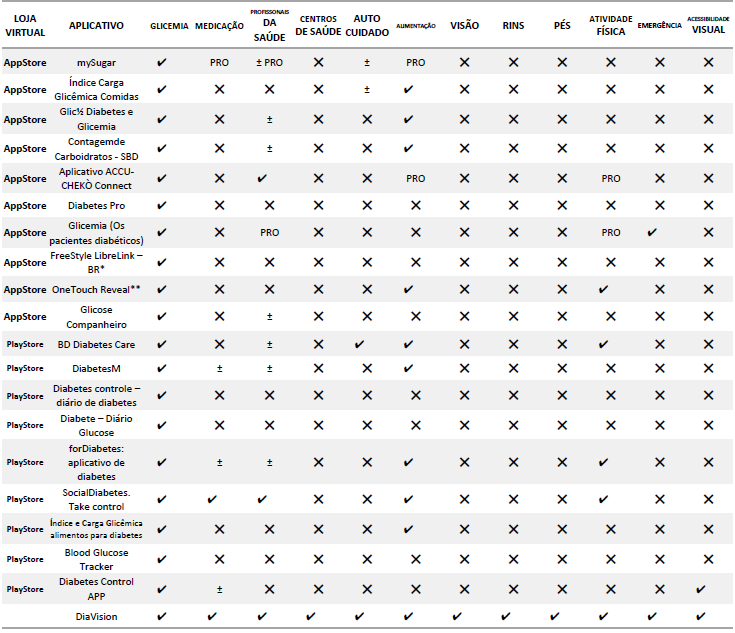
\includegraphics[scale=0.75]{Imagens/proposta/busca_anterioridade.png}
    \end{center}
    \legend{Fonte: \cite{Sobral2021}.}
\end{figure}

\newpage

\section{Visão e Análise}

Nesta seção são descritas as necessidades e características esperadas do produto de \emph{software} a ser desenvolvido, identificadas a partir de
reuniões com a dona do produto (PO, do inglês \emph{product owner}), esta que identificou a problemática abordada neste trabalho e
realizou o levantamento de funcionalidades e problemas das soluções já existentes no mercado em \citeonline{Sobral2021}.

\subsection{Descrição do Problema}

A \autoref{tab-desc-pro} apresenta, de forma resumida, o problema, seus impactos e a proposta de solução com seu diferencial.

\begin{table}[htb]
    \caption{Descrição do problema.}
    \label{tab-desc-pro}
    \begin{center}
        \begin{tabular}{p{4.0cm}|p{10.0cm}}
            \textbf{Problema}    & Dificuldade de acesso à informações de autocuidado com relação ao DM por deficientes visuais.                                          \\
            \hline
            \textbf{Afeta}       & Independência e qualidade de vida de diabéticos com DV\@.                                                                              \\
            \hline
            \textbf{Impacta}     & No autocuidado e, consequentemente, no controle do DM\@.                                                                               \\
            \hline
            \textbf{Solução}     & Desenvolvimento de aplicação móvel com conteúdos e funcionalidades que auxiliem diabéticos no gerenciamento do autocuidado com o DM\@. \\
            \hline
            \textbf{Diferencial} & Acessibilidade ao deficiente visual.
        \end{tabular}
    \end{center}
    \legend{Fonte: Autores.}
\end{table}

\subsection{Riscos e Impedimentos}

Os seguintes riscos e possíveis impedimentos com relação ao produto foram identificados:

\begin{itemize}
    \item Não adesão por parte do público alvo;
    \item Dificuldades no manuseio do \emph{smartphone} pelo público alvo;
    \item Dificuldade de localizar os possíveis participantes da pesquisa;
    \item Utilização incorreta do aplicativo ou não assimilação das informações adquiridas;
    \item Afastamento do paciente da assistência continuada na rede primária;
    \item Constrangimento do usuário por falta de entendimento das funcionalidades.
\end{itemize}

\newpage

\section{Requisitos}

Antes de inciar o desenvolvimento de qualquer tarefa técnica de engenharia de \emph{software}, é interessante que seja criado
um conjunto de requisitos.
Isso porque as tarefas de levantamento de requisitos levam a um entendimento dos impactos da solução, necessidades do cliente e
como os usuários finais vão interagir com o \emph{software}, diminuindo as chances de erros por má interpretação das solicitações
dos clientes \cite{pressman2014software}.

Esses requisitos costumam ser classificados como funcionais, não-funcionais e inversos \cite{sommerville2007engenharia}.
E serão apresentados nesta seção, iniciando pelas estórias de usuários, parte inicial do processo de elicitação
dos requisitos e finalizando com os casos de uso.

\newpage

\subsection{Estórias de usuários}

Estórias de usuários são muito utilizadas em metodologias ágeis e descrevem um cenário geral onde é possível visualizar
quais ações são possíveis, os atores envolvidos e quais os valores dessas ações, servindo como lembrete
de possíveis requisitos que precisam ser melhor detalhados com o cliente \cite{nawrocki2014agile}.

As estórias de usuários identificadas são listadas na \autoref{tab-est-usr}.

\begin{table}[htb]
    \begin{center}
        \ABNTEXfontereduzida
        \caption{Relação de estórias de usuários.}
        \label{tab-est-usr}
        \begin{tabular}{p{2.0cm}|p{5.0cm}|p{7.0cm}}
            %\hline
            \textbf{Eu, enquanto}                                          & \textbf{Quero} & \textbf{Para}                     \\
            \hline
            Paciente                                                       &
            Encontrar o \emph{app} nas lojas virtuais                      &
            Baixar o \emph{app} no meu celular.                                                                                 \\
            \hline
            Paciente                                                       &
            Realizar cadastro no aplicativo                                &
            Ter acesso às funcionalidades do \emph{app}.                                                                        \\
            \hline
            Paciente                                                       &
            Realizar login de forma prática                                &
            Para acessar as funcionalidades do \emph{app}.                                                                      \\
            \hline
            Paciente                                                       &
            Poder alterar minha senha                                      &
            Poder alterá\@-la e recuperar acesso ao \emph{app}.                                                                 \\
            \hline
            Paciente                                                       &
            Registrar informações das refeições                            &
            Acompanhar a quantidade de calorias consumidas por refeição.                                                        \\
            \hline
            Paciente                                                       &
            Ter acesso a aplicativos acessíveis para deficientes visuais   &
            Ajudar a realizar atividades do dia a dia.                                                                          \\
            \hline
            Paciente                                                       &
            Sugerir aplicativos acessíveis para deficientes visuais        &
            Compartilhar aplicativos que possam ajudar outros usuários com DV\@.                                                \\
            \hline
            Paciente                                                       &
            Registrar práticas de atividade física                         &
            Acompanhar a evolução da rotina de atividade física.                                                                \\
            \hline
            Paciente                                                       &
            Ter acesso à dicas de autocuidado                              &
            Melhorar a qualidade de vida e prevenir complicações do DM\@.                                                       \\
            \hline
            Paciente                                                       &
            Filtrar as dicas por categorias                                &
            Facilitar a busca das dicas sobre assuntos específicos.                                                             \\
            \hline
            Paciente                                                       &
            Consultar locais para acesso à serviços de saúde               &
            Facilitar o acesso e contato com as principais clínicas, hospitais e consultórios da cidade.                        \\
            \hline
            Paciente                                                       &
            Registrar glicemia                                             &
            Acompanhamento dos valores de glicemia e ser alertado quando estiver fora do limite.                                \\
            \hline
            Paciente                                                       &
            Registrar medicações que faço uso                              &
            Ter uma lista atualizada com todas as informações das medicações e ser alertado dos horários de uso das medicações. \\
            \hline
            Paciente                                                       &
            Realizar avaliação dos pés                                     &
            Acompanhar a evolução dos pés e detectar quando surgir alterações.                                                  \\
            \hline
            Paciente                                                       &
            Registrar diurese diária                                       &
            Acompanhar quando surgir alterações.                                                                                \\
            \hline
            Paciente                                                       &
            Ter acesso a relatórios dos dados registrados                  &
            Visualizar e compartilhar esses dados registrados.                                                                  \\
            \hline
            Paciente                                                       &
            Ter acesso aos dados pessoais                                  &
            Editar ou acrescentar dados pessoais durante o uso do aplicativo.                                                   \\
            \hline
            Paciente                                                       &
            Configurar notificações                                        &
            Definir horários e quais ativar ou desativar.                                                                       \\
            \hline
            Paciente                                                       &
            Configurar preferências                                        &
            Personalizar os limites da glicemia.                                                                                \\
            \hline
            Paciente                                                       &
            Realizar \emph{logout}                                         &
            Para desvincular minha conta do \emph{app}.                                                                         \\
            \hline
            Administrador do sistema                                       &
            Adicionar dicas de autocuidado para os pacientes               &
            Fornecer informações acerca de cuidados com a saúde.                                                                \\
            \hline
            Administrador do sistema                                       &
            Cadastrar centros de saúde no sistema                          &
            Que o paciente possa conhecer os centros de saúde que atendem suas demandas.                                        \\
            \hline
            Administrador do sistema                                       &
            Cadastrar sugestões de aplicativos acessíveis no sistema       &
            Que o paciente possa conhecer outros \emph{apps} acessíveis que possam ajudá\@-lo no cotiano.                       \\
            \hline
            Administrador do sistema                                       &
            Aprovar/recusar as sugestões de centros de saúde e aplicativos &
            Assegurar credibilidade ao aplicativo.                                                                              \\
            % \hline
        \end{tabular}
        \legend{Fonte: Autores.}
    \end{center}
\end{table}

\newpage

\subsection{Requisitos Funcionais}

A \autoref{tab-req-fun} mostra os requisitos funcionais da aplicação, estes que se referem, principalmente, às funções e 
comportamentos do sistema.

\begin{table}[htb]
    \begin{center}
        \ABNTEXfontereduzida
        \caption{Requisitos Funcionais da aplicação.}
        \label{tab-req-fun}
        \begin{tabular}{p{1.1cm}|p{1.3cm}|p{3.0cm}|p{1.5cm}|p{6.7cm}}
            %\hline
            \textbf{Código} & \textbf{Atores} & \textbf{Requisito}              & \textbf{Prioridade} & \textbf{Descrição} \\
            \hline
            RF01            & Paciente        & Manter paciente                 & Essencial           &
            O paciente poderá gerenciar seus dados na aplicação.                                                           \\
            \hline
            RF02            & Paciente        & Resetar senha                   & Essencial           &
            O paciente poderá solicitar a alteração de senha para recuperar acesso.                                        \\
            \hline
            RF03            & Paciente        & Autenticação                    & Essencial           &
            Será necessária autenticação com e-mail e senha para ter acesso às funcionalidades do \emph{app}.              \\
            \hline
            RF04            & Adminis-trador  & Manter Dicas de Autocuidado     & Essencial           &
            O administrador do sistema poderá gerenciar as dicas de autocuidado no sistema.                                \\
            \hline
            RF05            & Adminis-trador  & Manter Centros de Saúde         & Desejável           &
            O administrador do sistema poderá gerenciar os centros de saúde no sistema.                                    \\
            \hline
            RF06            & Adminis-trador  & Manter \emph{Apps} de Visão     & Importante          &
            O administrador do sistema poderá gerenciar sugestões de aplicativos acessíveis à PDV\@.                       \\
            \hline
            RF07            & Paciente        & Manter Registros de Diurese     & Importante          &
            O paciente poderá registrar diurese e gerenciar esses registros.                                               \\
            \hline
            RF08            & Paciente        & Manter Registros de Glicemia    & Essencial           &
            O paciente poderá registrar níveis de glicemia e gerenciar esses registros.                                    \\
            \hline
            RF09            & Paciente        & Manter Registros de Medicação   & Essencial           &
            O paciente poderá registrar suas medicações e gerenciar esses registros.                                       \\
            \hline
            RF10            & Paciente        & Manter Registros de Exercícios  & Importante          &
            O paciente poderá registrar atividades físicas realizadas e gerenciar esses registros.                         \\
            \hline
            RF11            & Paciente        & Manter Avaliações dos Pés       & Essencial           &
            O paciente poderá registrar avaliações do estado dos pés e gerenciar esses registros.                          \\
            \hline
            RF12            & Paciente        & Sugerir \emph{Apps} de Visão    & Importante          &
            O paciente poderá sugerir de aplicativos acessíveis à PDV para avaliação do administrador.                     \\
            \hline
            RF13            & Paciente        & Manter Registros de Alimentação & Essencial           &
            O paciente poderá registrar os alimentos que consumiu por refeição e gerenciar esses registros.                \\
            \hline
            RF14            & Paciente        & Consultar Dicas de Autocuidado  & Essencial           &
            O paciente poderá consultar as dicas de autocuidado disponíveis no sistema.                                    \\
            \hline
            RF15            & Paciente        & Consultar Centros de Saúde      & Desejável           &
            O paciente poderá consultar os centros de saúde disponíveis no sistema.                                        \\
            \hline
            RF16            & Paciente        & Consultar \emph{Apps} de Visão  & Importante          &
            O paciente poderá consultar sugestões de aplicativos acessíveis à PDV\@ disponíveis no sistema.                \\
            \hline
            RF17            & Paciente        & Sugerir Centros de Saúde        & Desejável           &
            O paciente poderá sugerir centros de saúde para avaliação do administrador.                                    \\
            \hline
            RF18            & Paciente        & Configurar Notificações         & Essencial           &
            O paciente poderá configurar quais notificações deseja receber e os horários.                                  \\
            \hline
            RF19            & Paciente        & Envio de Notificações           & Essencial           &
            Notificações deverão ser enviadas de acordo com as configurações definidas pelo paciente.                      \\
            % \hline
        \end{tabular}
        \legend{Fonte: Autores.}
    \end{center}
\end{table}

\newpage

\subsection{Requisitos Não-Funcionais}

Requisitos não-funcionais em sistemas podem ser descritos como atributos de qualidade, desempenho, segurança ou gerais, estes que podem
ser identificados a partir das necessidades do cliente mesmo que não tenham sido falados explicitamente \cite{pressman2014software}.

Assim, na \autoref{tab-req-nf}, são listados esses requisitos identificados juntamente com o tipo e a prioridade
de cada um deles para este projeto.

\begin{table}[htb]
    \begin{center}
        \ABNTEXfontereduzida
        \caption{Requisitos Não-Funcionais da aplicação.}
        \label{tab-req-nf}
        \begin{tabular}{p{1.1cm}|p{1.6cm}|p{3.0cm}|p{1.5cm}|p{6.7cm}}
            %\hline
            \textbf{Código} & \textbf{Tipo} & \textbf{Requisito}              & \textbf{Prioridade} & \textbf{Descrição} \\
            \hline
            RNF01           & Usabilidade   & Acessibilidade                  & Essencial           &
            Implementar as técnicas de acessibilidade para solucionar os principais problemas relacionados.              \\
            \hline
            RNF02           & Usabilidade   & Simplicidade                    & Essencial           &
            \emph{Interface} simples e intuitiva, mantendo apenas as informações necessárias na tela.                    \\
            \hline
            RNF03           & Usabilidade   & Buscas Ágeis                    & Desejável           &
            Facilitar buscas por meio de \emph{auto complete}.                                                           \\
            \hline
            RNF04           & Segurança     & Compartilhamento de Informações & Essencial           &
            Somente o próprio usuário terá acesso e poderá compartilhar suas informações.                                \\
            \hline
            RNF05           & Tecnologia    & Aplicação multiplataforma       & Desejável           &
            Deve-se utilizar de ferramentas que possibilitem a construção da aplicação para Android e iOS\@.             \\
            % \hline
        \end{tabular}
        \legend{Fonte: Autores.}
    \end{center}
\end{table}

\subsection{Requisitos Inversos}

Os requisitos listados na \autoref{tab-req-inv}, chamados inversos, se referem às restrições, condições que não devem ocorrer no sistema.

\begin{table}[htb]
    \begin{center}
        \ABNTEXfontereduzida
        \caption{Requisitos Inversos da aplicação.}
        \label{tab-req-inv}
        \begin{tabular}{p{1.1cm}|p{1.5cm}|p{10.5cm}}
            %\hline
            \textbf{Código} & \textbf{Prioridade} & \textbf{Descrição}         \\
            \hline
            RI01            & Essencial           &
            Um usuário não deve poder acessar recursos de outros.              \\
            \hline
            RI02            & Essencial           &
            Os usuários não devem ser notificados se não estiverem deslogados. \\
            \hline
            RI03            & Essencial           &
            O administrador do sistema não deve ter acesso aos dados dos usuários.
            % \hline
        \end{tabular}
        \legend{Fonte: Autores.}
    \end{center}
\end{table}

\newpage

\subsection{Casos de Uso}

De acordo com \citeonline{pressman2014software}, um caso de uso é caracterizado como um ``contrato de comportamento'' que define como
um ator utiliza um sistema para alcançar algum objetivo e descreve um cenário de uso de forma simples do ponto de vista desse ator.

A partir dos requisitos e estórias de usuários identificados, o diagrama de casos de usos da \autoref{fig_use_cas} foi elaborado.

\begin{figure}[htb]
    \caption{\label{fig_use_cas}Diagrama de casos de uso.}
    \begin{center}
        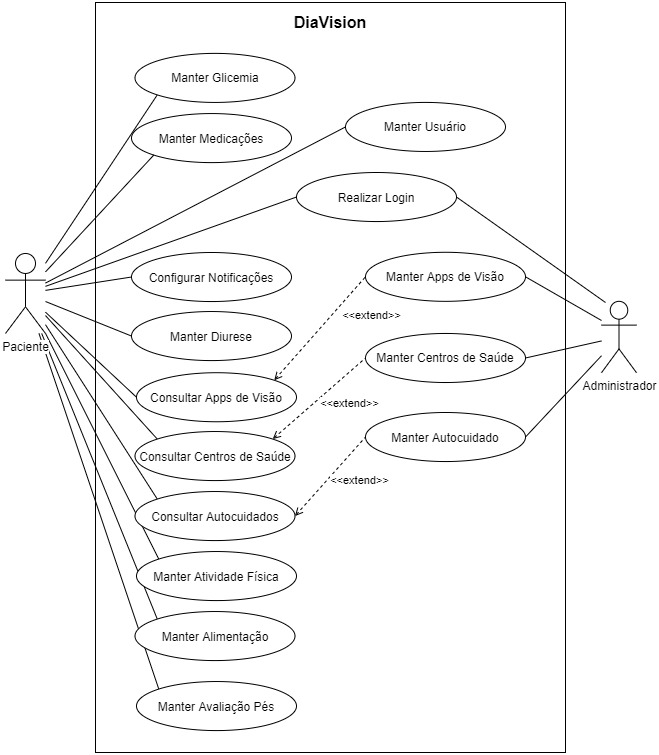
\includegraphics[scale=0.65]{Imagens/proposta/use_case.jpg}
    \end{center}
    \legend{Fonte: Autor.}
\end{figure}

\newpage

\section{Protótipo de Telas}

Nesta seção são apresentadas imagens do protótipo de telas elaborado no estudo \citeonline{Sobral2021}, com o objetivo de melhorar o entendimento dos
requisitos e funcionalidades do aplicativo que será desenvolvido.
Assim, nas \autoref{fig_tel_ini_prot} e \autoref{fig_tel_pos_prot} são mostradas as telas iniciais e demais telas do protótipo.

\begin{figure}[htb]
    \caption{\label{fig_tel_ini_prot}Telas iniciais do protótipo.}
    \begin{center}
        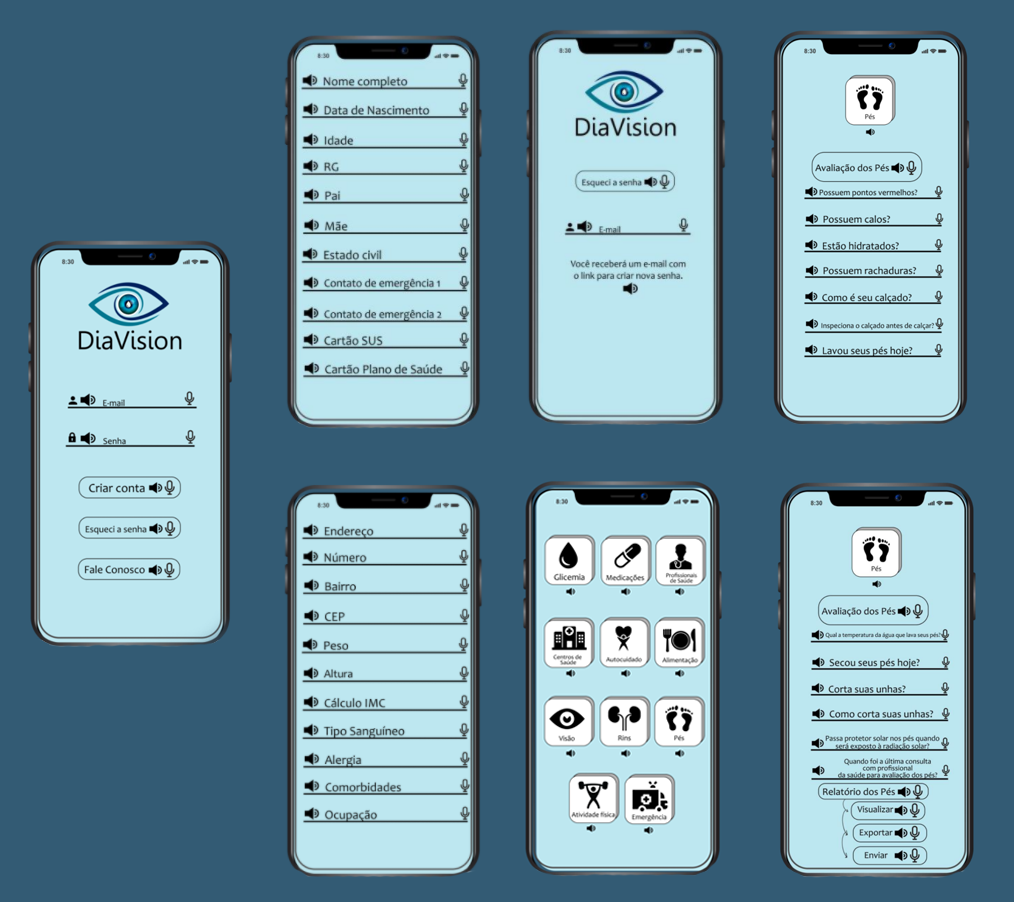
\includegraphics[scale=0.57]{Imagens/proposta/telas_iniciais_prot.png}
    \end{center}
    \legend{Fonte: \cite{Sobral2021}.}
\end{figure}

\begin{figure}[htb]
    \caption{\label{fig_tel_pos_prot}Demais telas do protótipo.}
    \begin{center}
        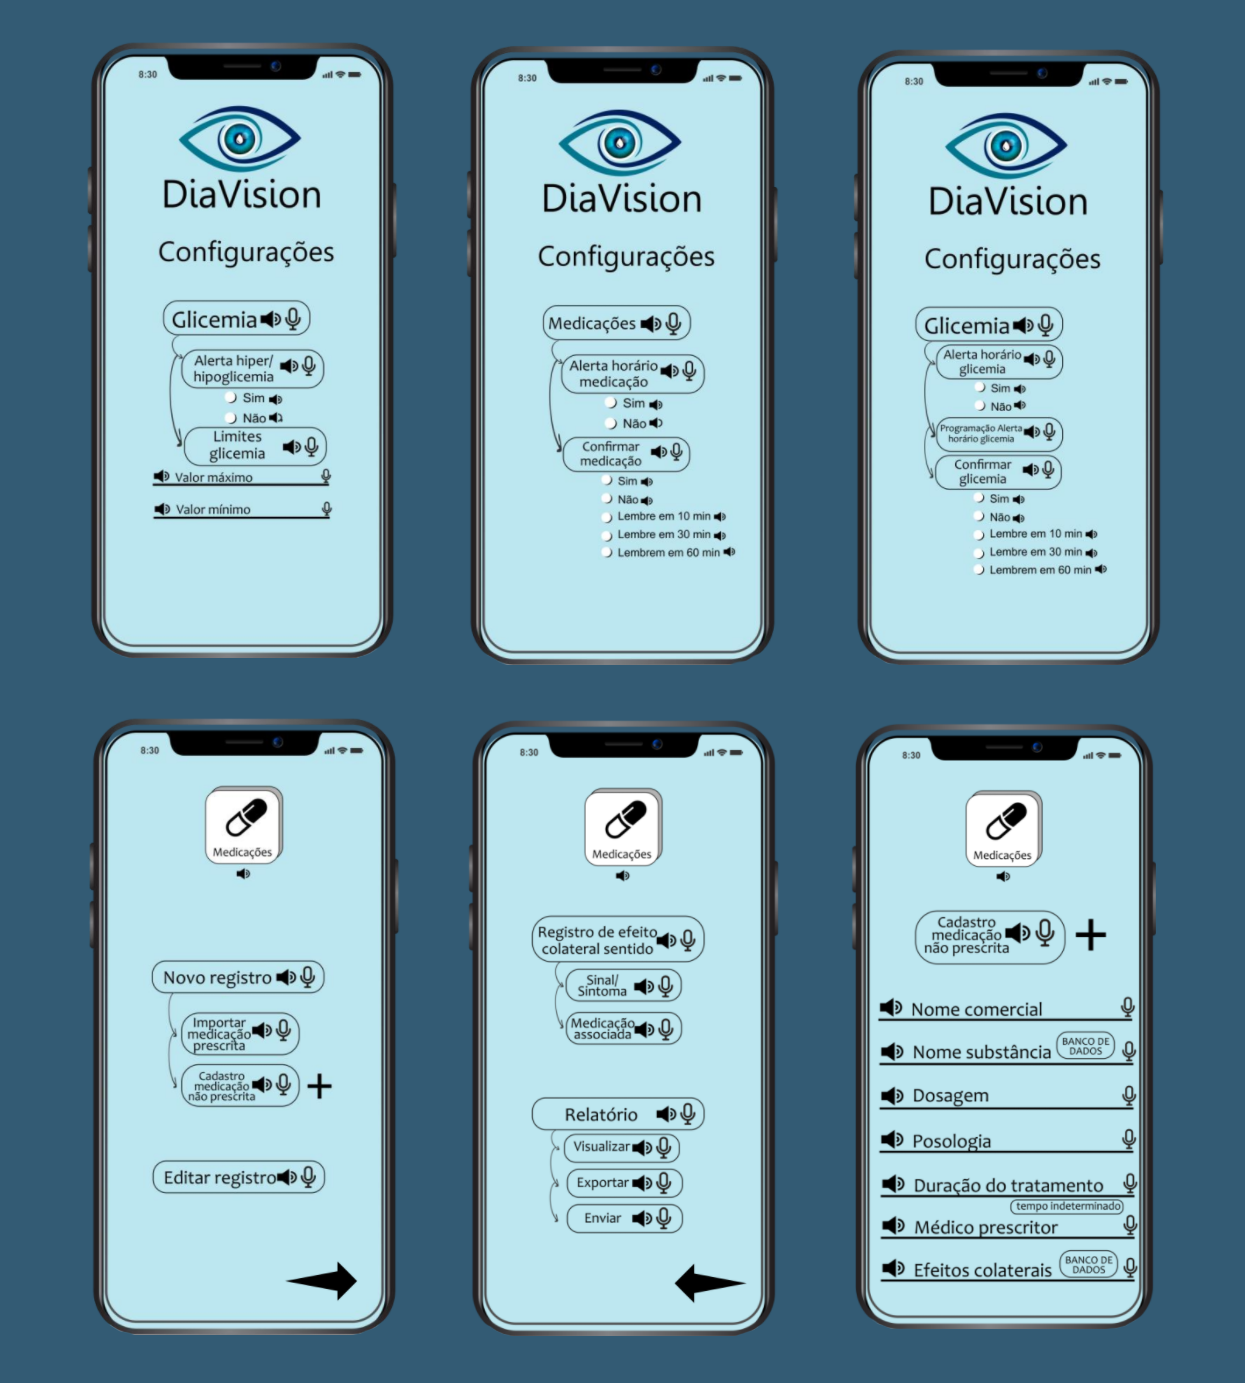
\includegraphics[scale=0.45]{Imagens/proposta/telas_post_prot.png}
    \end{center}
    \legend{Fonte: \cite{Sobral2021}.}
\end{figure}

\newpage

\section{Cronograma}

Por fim, o cronograma na \autoref{fig_cro_con} foi definido visando a organização e planejamento das atividades que serão realizadas
na segunda parte desse trabalho.

\begin{figure}[htb]
    \caption{\label{fig_cro_con}Cronograma de continuidade do Projeto.}
    \begin{center}
        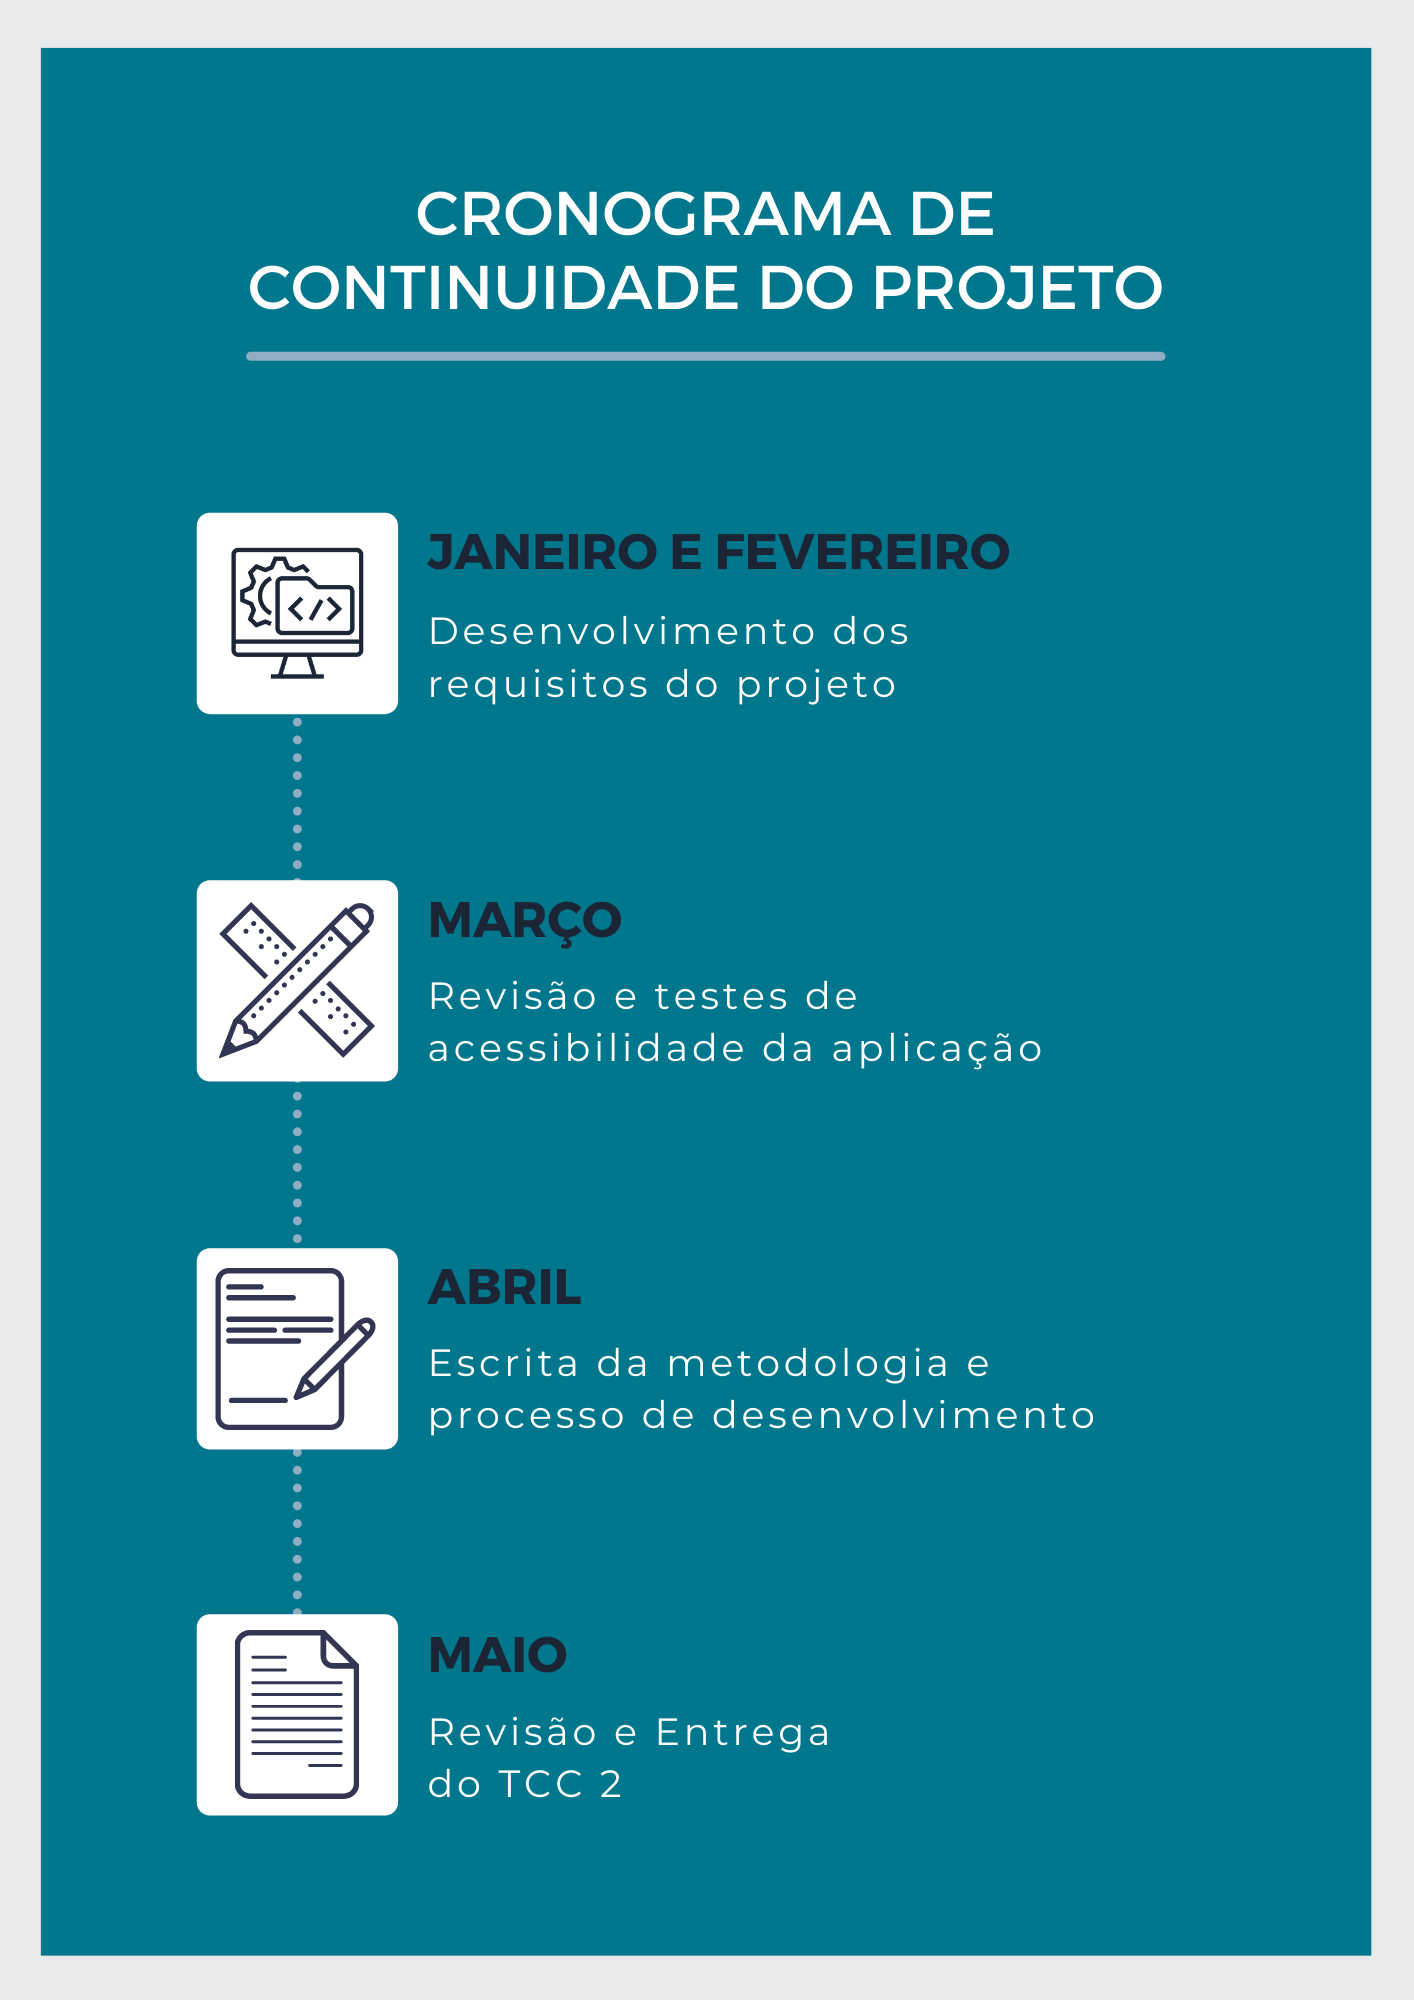
\includegraphics[scale=0.65]{Imagens/proposta/cronograma_continuidade.png}
    \end{center}
    \legend{Fonte: Autor.}
\end{figure}
% \chapter{Considerações Finais}
\label{ch:conclusion}

Este trabalho buscou contextualizar e fundamentar a problemática identificada pela dificuldade
no acesso à informações sobre o autocuidado com o DM por pacientes com DV\@. Para isso, foram introduzidos
o DM e suas complicações relacionadas à DV, bem como, foram apresentados dados que indicam o crescimento no
número de casos de ambos.

Por meio de estudos anteriores, em um trabalho de mestrado que acarretou na parceira para desenvolvimento deste
projeto, foi possível um aprofundamento sobre as necessidades e requisitos do público-alvo.
Onde foram identificadas a importância do autocuidado no tratamento do DM e as principais funcionalidades utilizadas
como solução no mercado \cite{Sobral2021}.

Outra problemática introduzida foi que, mesmo com o aumento da informatização e popularização dos \emph{smartphones},
PDV ainda enfrentam sérios problemas quanto à falta de acessibilidade à DV em aplicações móveis \cite{Shera2021285}.
E apontadas as principais ferramentas e diretrizes relacionadas à acessibilidade disponibilizadas pelas plataformas móveis.

Assim, foi realizado um processo de MSL visando identificar as principais soluções que estão sendo adotadas
para essa problemática. Nesse processo de mapeamento, foram extraídas informações relevantes
de trabalhos publicados em bases acadêmicas que apresentaram técnicas para resolver esses problemas
em aplicações móveis.

A partir da análise dos resultados do MSL, estabeleceram-se as técnicas de acessibilidade que seriam utilizadas
na solução proposta, sendo apresentados o planejamento e cronograma de continuidade de seu desenvolvimento.

Concluímos que o autocuidado pode ajudar a reduzir significativamente as complicações ocasionadas pelo DM \cite{ADA2019}.
Assim, aliando-o ao crescimento no acesso à Internet por meio de \emph{smartphones}, de acordo com \citeonline{CETIC_2021},
e à aplicação das principais técnicas para resolução dos problemas de acessibilidade em aplicativos móveis, propomos o
desenvolvimento de uma aplicação fruto da combinação de todas essas características.

\phantompart
\bibliography{Bibliografia}

%%%%%%%%%%%%%%%%%%%%%%%%%%%%%%%%%%%%%%%%%%%%%%%%%%%%%%%%%%%%%%%%%%%%%%%%%%
% ELEMENTOS PÓS-TEXTUAIS
%%%%%%%%%%%%%%%%%%%%%%%%%%%%%%%%%%%%%%%%%%%%%%%%%%%%%%%%%%%%%%%%%%%%%%%%%%

%\postextual

\renewcommand{\chapnumfont}{\chaptitlefont}
\renewcommand{\afterchapternum}{}
%\include{Pos_Textual/Apendices}
%\include{Pos_Textual/Anexos}

\end{document}